%%%%%%%%%%%%%%%%%%%%%%%%%%%%%%%%%%%%%%%%%
% Thin Sectioned Essay
% LaTeX Template
% Version 1.0 (3/8/13)
%
% This template has been downloaded from:
% http://www.LaTeXTemplates.com
%
% Original Author:
% Nicolas Diaz (nsdiaz@uc.cl) with extensive modifications by:
% Vel (vel@latextemplates.com)
%
% License:
% CC BY-NC-SA 3.0 (http://creativecommons.org/licenses/by-nc-sa/3.0/)
%
%%%%%%%%%%%%%%%%%%%%%%%%%%%%%%%%%%%%%%%%%

%----------------------------------------------------------------------------------------
%	PACKAGES AND OTHER DOCUMENT CONFIGURATIONS
%----------------------------------------------------------------------------------------

\documentclass[a4paper, 12pt]{article} % Font size (can be 10pt, 11pt or 12pt) and paper size (remove a4paper for US letter paper)
\usepackage[portuguese]{babel}

\usepackage[protrusion=true,expansion=true]{microtype} % Better typography
\usepackage{graphicx} % Required for including pictures
\usepackage{wrapfig} % Allows in-line images

\usepackage{hyperref}%Required for hyperlink references
\hypersetup{
	colorlinks=true, % Ativa links coloridos em vez de caixas ao redor
	linkcolor=black, % Cor dos links internos
	citecolor=black, % Cor das citações
	urlcolor=black   % Cor dos links externos (Jira, por exemplo)
}

\usepackage{mathpazo} % Use the Palatino font
\usepackage[T1]{fontenc} % Required for accented characters
\linespread{1.05} % Change line spacing here, Palatino benefits from a slight increase by default
\usepackage{float}
\usepackage[backend=bibtex,style=numeric]{biblatex}
\addbibresource{references.bib} % Nome do arquivo de referências
\makeatletter
\renewcommand\@biblabel[1]{\textbf{#1.}} % Change the square brackets for each bibliography item from '[1]' to '1.'
\renewcommand{\@listI}{\itemsep=0pt} % Reduce the space between items in the itemize and enumerate environments and the bibliography

\renewcommand{\maketitle}{
\begin{titlepage}
\begin{center}
\vspace*{1cm}

\includegraphics[width=0.35\textwidth]{../images/logo-no-bg.png}\\[1cm] % Logo
{\Huge\textbf{Vizzy - Plataforma Comunitária}}\\[0.5cm] % Main Title
{\Large Projeto de Desenvolvimento de Software}\\[2cm] % Subtitle
{\large \textsc{
	Enrique Rodrigues Nº28602 \\
	José Alves Nº27967 \\
	Diogo Machado Nº26042 \\
	Diogo Abreu Nº27975 \\
	André Silva Nº27965}}\\[0.5cm] % Authors
{\textit{Instituto Politécnico do Cávado e do Ave}}\\[1.5cm] % Institution
{\large \today} % Date
\vfill
% \textbf{Keywords:} lorem, ipsum, dolor, sit amet, lectus % Keywords
\end{center}
\end{titlepage}
}
\makeatother

%----------------------------------------------------------------------------------------
%	TITLE
%----------------------------------------------------------------------------------------

\title{\textbf{Vizzy - Plataforma Comunitária}\\ % Title
	Projeto de Desenvolvimento de Software} % Subtitle

\author{
	\textsc{Enrique Rodrigues Nº28602}, \\
	\textsc{José Alves}, \\
	\textsc{Diogo Machado}, \\
	\textsc{Diogo Abreu Nº27975}, \\ 
	\textsc{André Silva} \\
	\textit{Instituto Politécnico do Cávado e do Ave}
}

\date{\today} % Date

%------------------------------------------------------------------------------------

\begin{document}
\maketitle % Print the title section

%----------------------------------------------------------------------------------------
%	ABSTRACT AND KEYWORDS
%----------------------------------------------------------------------------------------

%\renewcommand{\abstractname}{Summary} % Uncomment to change the name of the abstract to something else

% \begin{abstract}
% Morbi tempor congue porta. Proin semper, leo vitae faucibus dictum, metus mauris lacinia lorem, ac congue leo felis eu turpis. Sed nec nunc pellentesque, gravida eros at, porttitor ipsum. Praesent consequat urna a lacus lobortis ultrices eget ac metus. In tempus hendrerit rhoncus. Mauris dignissim turpis id sollicitudin lacinia. Praesent libero tellus, fringilla nec ullamcorper at, ultrices id nulla. Phasellus placerat a tellus a malesuada.
% \end{abstract}

% \hspace*{3,6mm}\textit{Keywords:} lorem , ipsum , dolor , sit amet , lectus % Keywords

% \vspace{30pt} % Some vertical space between the abstract and first section

%----------------------------------------------------------------------------------------
%	DOCUMENT BODY
%----------------------------------------------------------------------------------------

\newpage
\renewcommand{\contentsname}{Índice}
\tableofcontents

%------------------------------------------------------------------------------------

\newpage
\renewcommand{\listfigurename}{Lista de Figuras}
\listoffigures

%------------------------------------------------------------------------------------

\newpage
\section{Introdução}

A \textit{Vizzy} é uma plataforma comunitária desenvolvida para facilitar a compra, venda, troca e aluguer de itens entre pessoas da mesma comunidade, promovendo uma forma prática, económica e sustentável de partilhar recursos.

Através da \textit{Vizzy}, os utilizadores podem adquirir produtos em segunda mão, trocar itens ou até alugar ferramentas, entre outras coisas. Isto não só reduz o desperdício, como também oferece uma alternativa mais acessível, especialmente quando se trata de alugueres. Alugar uma máquina a um vizinho, por exemplo, pode ser muito mais económico do que comprá-la.

\subsection{Objetivo}
O objetivo da plataforma é criar uma rede de partilha dentro de uma comunidade, onde os membros possam beneficiar de um consumo mais consciente, poupando dinheiro e recursos, enquanto promovem a sustentabilidade e a cooperação.

Neste relatório, serão apresentados os principais detalhes da aplicação, incluindo diagramas UML e \textit{mockups}, que ilustram as funcionalidades essenciais da \textit{Vizzy}.

\subsection{Gestão do Projeto}
O \textit{Product Backlog}, as \textit{Sprints} e as \textit{Issues} podem ser consultados através do \href{https://ipcapt-my.sharepoint.com/:x:/g/personal/nfr\_ipca\_pt/Eb29k3z-aWRGisXGIZopL6IBy5l5QZjY8SjG1iWQDl6c7w?rtime=jE\_b04Za3Ug}{\textbf{Documento Excel}} ou do \href{https://basigraphics.atlassian.net/jira/software/projects/VIZZY/boards/1/backlog?epics=visible&atlOrigin=eyJpIjoiOGNmZTQ2MDRmNjQ1NDY0NDgwNDk0MDJiMGM0MDdlZWYiLCJwIjoiaiJ9}{\textbf{Jira Board}}. O código-fonte do projeto está disponível no \href{https://github.com/Basiiii/Vizzy}{\textbf{Repositório GitHub}}.

%------------------------------------------------------------------------------------

\newpage
\section{Problema e Motivação}

\subsection{O Problema}

Nos dias de hoje, muitas comunidades enfrentam desafios económicos e ambientais relacionados com o consumo excessivo e a falta de acesso a certos produtos. Itens valiosos acabam por ser desperdiçados ou ficam esquecidos, enquanto outras pessoas na mesma comunidade poderiam beneficiar deles. Ao mesmo tempo, a aquisição de novos produtos nem sempre é uma opção viável devido ao custo ou à disponibilidade limitada.

Outro desafio importante é a falta de soluções práticas para facilitar a troca, venda e aluguer de itens de forma organizada, o que leva a um ciclo de consumo ineficiente e ao desperdício de recursos.

\subsection{A Solução Proposta}

A \textit{Vizzy} surge como uma resposta a estes problemas, oferecendo uma plataforma onde os membros da comunidade podem comprar, vender, trocar e alugar itens de forma simples e segura. Com esta solução, é possível dar uma segunda vida a produtos que seriam descartados e permitir que as pessoas acedam a bens de que necessitam, sem precisarem de comprá-los novos.

Além disso, ao permitir o aluguer de ferramentas e outros objectos, a \textit{Vizzy} oferece uma alternativa económica e prática, como no caso de alugar uma ferramenta a um vizinho em vez de recorrer a serviços externos ou grandes empresas. Isto não só reduz os custos para os utilizadores, mas também contribui para um modelo de consumo mais sustentável.

A plataforma visa, assim, otimizar o uso dos recursos, reduzir desperdícios e fortalecer os laços entre membros da comunidade. Com a \textit{Vizzy}, todos podem beneficiar de uma forma mais acessível e consciente de consumir, promovendo a circulação de bens e a sustentabilidade.

%------------------------------------------------------------------------------------

\newpage
\section{Processos de Negócio}

\subsection{Processo de Empréstimo/Aluguer}

\subsubsection{Etapas}
\begin{itemize}
	\item \textbf{Criar um anúncio}: O utilizador cria um anúncio na plataforma, fornecendo detalhes como o produto que pretende alugar/emprestar, descrição do mesmo, estado e fotografias.
	\item \textbf{Definir datas bloqueadas}: O utilizador indica, caso existam, as datas em que o produto não estará disponível para empréstimo/aluguer.
	\item \textbf{Confirmar datas livres}: O sistema verifica e confirma as datas disponíveis para empréstimo/aluguer com base nas datas bloqueadas.
	\item \textbf{Definir valor associado}: O utilizador define o valor do aluguer (0€ em caso de empréstimo).
	\item \textbf{O anúncio não desaparece}: Durante o empréstimo/aluguer, o anúncio permanece na plataforma para futuras marcações.
\end{itemize}

\subsubsection{Fluxo do Processo}
Um utilizador cria o anúncio e define as datas indisponíveis (fazendo o sistema a gestão das datas disponíveis, com base nesta informação). Outros utilizadores podem solicitar o empréstimo/aluguer do produto nas datas livres. O proprietário do produto confirma ou rejeita a solicitação. O anúncio continua a estar disponível na plataforma para marcações em datas livres.

\subsubsection{Interações Essenciais}
\begin{itemize}
	\item Possibilidade de enviar uma contra-proposta no anúncio. Por exemplo, em vez de alugar um corta-relva, o utilizador pode sugerir emprestar um soprador.
\end{itemize}

\subsection{Processo de Venda}

\subsubsection{Etapas}
\begin{itemize}
	\item \textbf{Criar um anúncio}: O utilizador cria um anúncio na plataforma, fornecendo detalhes como o produto que pretende vender, descrição do mesmo, estado e fotografias.
	\item \textbf{Definir um valor associado}: O utilizador define o preço de venda do produto (0€, no caso de ser um \textit{giveaway}).
	\item \textbf{Permitir ou não receber contrapropostas}: O utilizador decide se aceita ou não receber contrapropostas de outros utilizadores.
	\item \textbf{Aceitar/Rejeitar contrapropostas}: Caso permita, o vendedor pode aceitar ou rejeitar contrapropostas recebidas.
	\item \textbf{Concretizada a venda, o anúncio desaparece}: Após a venda, o anúncio é marcado como concluído, deixando de aparecer nas pesquisas.
\end{itemize}

\subsubsection{Fluxo do Processo}
O utilizador cria o anúncio e define o preço. Outros utilizadores podem comprar diretamente ou fazer contrapropostas (se permitido pelo vendedor). O vendedor aceita, rejeita ou faz ele uma nova contraproposta. Após a venda, o anúncio é removido das pesquisas, ficando guardado para efeitos de histórico.

\subsection{Processo de Troca}

\subsubsection{Etapas}
\begin{itemize}
	\item \textbf{Criar um anúncio}: O utilizador cria um anúncio na plataforma, fornecendo detalhes como o produto que pretende vender, descrição do mesmo, estado e fotografias.
	\item \textbf{Associar um produto para troca}: O utilizador indica que produto deseja receber em troca.
	\item \textbf{Aceitar a proposta}: Outros utilizadores podem aceitar a proposta, oferecendo o produto solicitado.
	\item \textbf{Fazer contrapropostas}: Outros utilizadores podem fazer contrapropostas com produtos diferentes.
	\item \textbf{Aceitar/Rejeitar contrapropostas}: O utilizador pode aceitar ou rejeitar as contrapropostas recebidas.
\end{itemize}

\subsubsection{Fluxo do Processo}
O utilizador cria o anúncio e indica o produto que deseja receber em troca. O utilizador aceita ou rejeita as contrapropostas recebidas. Após a troca, o anúncio é removido das pesquisas.

\subsection{Fluxo Geral}
\begin{itemize}
	\item O utilizador escolhe o tipo de transação (empréstimo/aluguer, venda ou troca).
	\item O utilizador cria o anúncio e define os detalhes específicos para cada processo.
	\item Outros utilizadores interagem com o anúncio (solicitam empréstimo, compram ou propõem trocas).
	\item O proprietário do produto confirma ou rejeita as solicitações.
	\item Após a transação, o anúncio é marcado como concluído (no caso da venda).
	\item No caso de empréstimo/aluguer, o anúncio permanece disponível, com as datas disponíveis atualizadas.
\end{itemize}

%------------------------------------------------------------------------------------

\newpage
\section{Requisitos Funcionais}
Os requisitos funcionais \textbf{(RFs)} são as especificações que definem o que um sistema deve fazer para atender às necessidades dos utilizadores. Eles descrevem as funcionalidades, comportamentos e operações que o sistema deve oferecer, incluindo interações entre utilizadores e o sistema, processamento de dados e regras de negócio.

\begin{table}[H]
	\centering
	\renewcommand{\arraystretch}{1.3}
	\begin{tabular}{|c|p{12cm}|}
		\hline
		\textbf{Código} & \textbf{Requisito Funcional} \\
		\hline
		\textbf{RF 01} & O utilizador pode criar um anúncio na aplicação, fornecendo nome, descrição, estado do produto, fotografias e definir se é para venda, troca ou empréstimo/aluguer. \\
		\hline
		\textbf{RF 02} & O utilizador pode definir datas bloqueadas para empréstimo/aluguer do produto. \\
		\hline
		\textbf{RF 03} & O sistema deve verificar e confirmar as datas livres para empréstimo/aluguer. \\
		\hline
		\textbf{RF 04} & O utilizador pode definir um valor para aluguer ou venda. \\
		\hline
		\textbf{RF 05} & O utilizador pode permitir ou não propostas nos anúncios. \\
		\hline
		\textbf{RF 06} & O utilizador pode aceitar, rejeitar ou negociar propostas. \\
		\hline
		\textbf{RF 07} & Após a transação de um produto para venda ou troca, o anúncio deve ser marcado como concluído e deixar de aparecer para os outros utilizadores. \\
		\hline
		\textbf{RF 08} & O utilizador, ao criar um anúncio para troca, pode indicar qual produto deseja receber em troca. \\
		\hline
		\textbf{RF 09} & A aplicação deve permitir a pesquisa de produtos disponíveis na plataforma. \\
		\hline
		\textbf{RF 10} & O utilizador pode adicionar produtos a uma lista de desejos/favoritos. \\
		\hline
	\end{tabular}
	\caption{Requisitos Funcionais}
	\label{tab:requisitos_funcionais}
\end{table}

%------------------------------------------------------------------------------------

\newpage
\section{Requisitos Não Funcionais}

Os requisitos não funcionais \textbf{(RNFs)} definem as características e restrições de um sistema que não estão diretamente relacionadas com as funcionalidades oferecidas, mas sim à qualidade, desempenho, segurança e usabilidade da aplicação. Eles garantem que o sistema seja eficiente, confiável e utilizável dentro de determinados padrões.

\begin{table}[H]
	\centering
	\renewcommand{\arraystretch}{1.3}
	\begin{tabular}{|c|p{12cm}|}
		\hline
		\textbf{Código} & \textbf{Requisito Não Funcional} \\
		\hline
		\textbf{RNF 01} & A interface do utilizador deve ser intuitiva e acessível para todas as faixas etárias. \\
		\hline
		\textbf{RNF 02} & Todos os dados dos utilizadores devem ser armazenados de forma segura. \\
		\hline
		\textbf{RNF 03} & A aplicação deve cumprir com o Regulamento Geral de Proteção de Dados (RGPD) da União Europeia, garantindo a privacidade e o consentimento para o uso de dados pessoais. \\
		\hline
		\textbf{RNF 04} & O tempo de carregamento do feed da aplicação não deve ultrapassar os 3 segundos. \\
		\hline
		\textbf{RNF 05} & A pesquisa de produtos deve devolver os resultados em menos de 5 segundos.\\
		\hline
		\textbf{RNF 06} & O sistema deve permitir a implementação de novas funcionalidades com um impacto mínimo no desempenho. \\
		\hline
		\textbf{RNF 07} & A aplicação deve exigir uma palavra-passe com pelo menos 8 caracteres, incluindo letras e números. \\
		\hline
		\textbf{RNF 08} & O sistema deve utilizar armazenamento em cache para reduzir o número de pedidos ao servidor e melhorar a eficiência. \\
		\hline
		\textbf{RNF 09} & O sistema deve limitar o tamanho máximo de imagens carregadas para 5MB, evitando uso excessivo de espaço. \\
		\hline
	\end{tabular}
	\caption{Requisitos Não Funcionais}
	\label{tab:requisitos_nao_funcionais}
\end{table}

%------------------------------------------------------------------------------------

\newpage

\section{Arquitetura}
A arquitetura da plataforma é composta por um \textit{frontend} desenvolvido com \textbf{React e Next.js}, um \textit{backend} em \textbf{C\#}, e uma base de dados gerida com \textbf{Supabase (PostgreSQL)}. Esta abordagem garante um sistema eficiente, seguro e escalável.

\begin{figure}[ht]
	\centering
	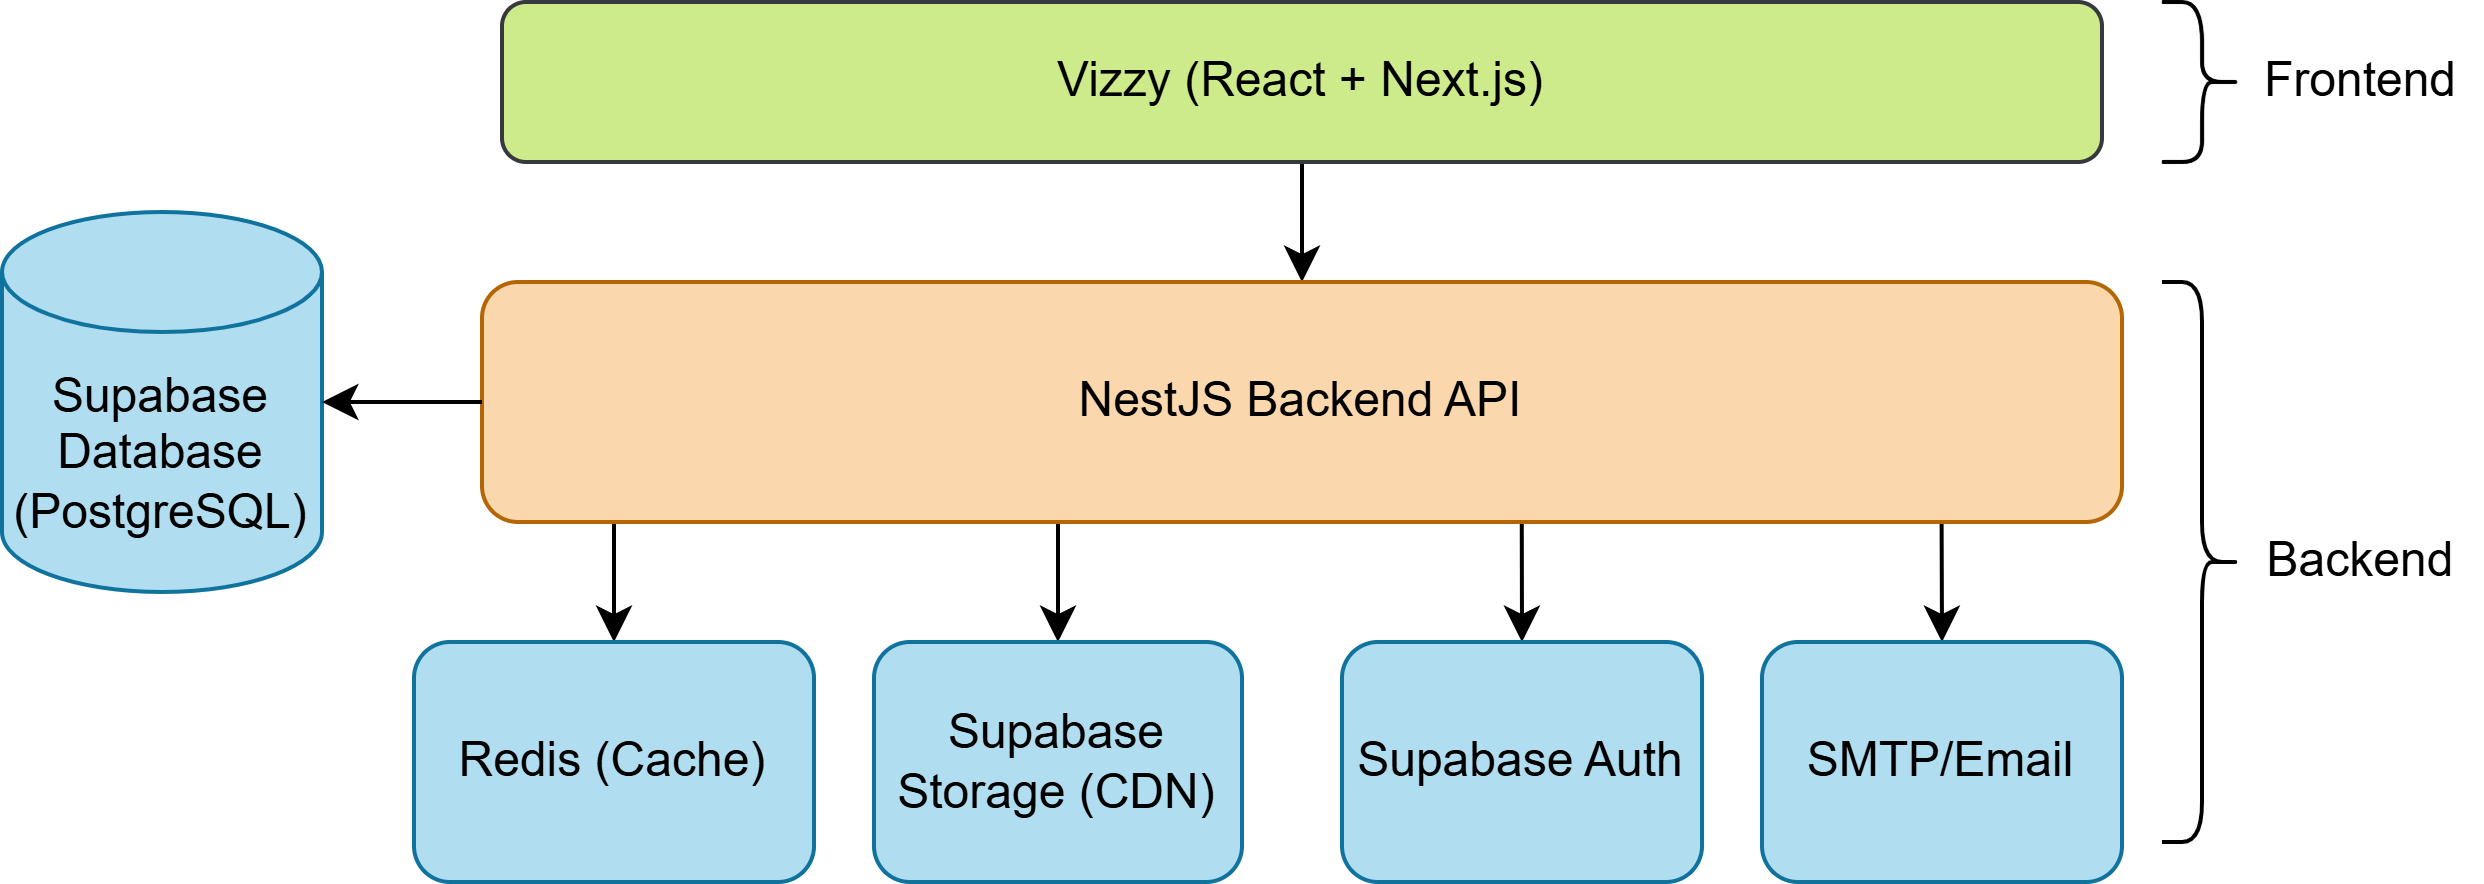
\includegraphics[width=\textwidth]{../images/system-architecture.png}
	\caption{Arquitetura da Plataforma}
	\label{fig:arquitetura}
\end{figure}

\subsection{Frontend}
O \textit{frontend} foi desenvolvido com \textbf{Next.js} para tirar proveito do \textit{server-side rendering} (SSR) e \textit{static site generation} (SSG), o que melhora o desempenho e o SEO. O frontend comunica diretamente com o \textbf{API Backend (C\#)}, chamando os endpoints para obter e manipular dados.

\subsection{Backend}
O \textit{backend} é composto por diversos serviços que trabalham em conjunto para garantir a funcionalidade da plataforma:

\begin{itemize}
	\item \textbf{API Backend (C\#):} Responsável pelo processamento dos pedidos HTTP do \textit{frontend}, gestão de dados e comunicação com a base de dados. A API também implementa caching com \textbf{Redis} para melhorar o desempenho, reduzindo a carga na base de dados e melhorando o tempo de resposta.
	\item \textbf{Redis (Cache):} Utilizado para guardar em cache respostas frequentes da API e melhorar a eficiência do sistema.
	\item \textbf{Supabase Auth:} Sistema de autenticação e gestão de utilizadores, garantindo segurança no acesso à plataforma.
	\item \textbf{SMTP/Email:} Serviço de envio de emails para recuperação de conta.
	\item \textbf{Supabase Storage (CDN):} Responsável por armazenar ficheiros e gerir recursos estáticos. A API busca os URLs dos ficheiros armazenados e devolve-os ao chamador da API.
\end{itemize}

\subsection{Base de Dados}
A plataforma utiliza o \textbf{PostgreSQL} como base de dados relacional. Esta base de dados oferece alta escalabilidade, confiabilidade e desempenho, permitindo operações eficientes de leitura e escrita.

\subsection{Fluxo de Funcionamento}
\begin{enumerate}
	\item O utilizador interage com o \textbf{frontend (Vizzy)}.
	\item Os pedidos são enviados para o \textbf{API Backend (C\#)}, que os processa e consulta a base de dados. Para melhorar o desempenho, o \textbf{Redis} atua como cache, guardando dados frequentes. Isto reduz consultas repetitivas à base de dados.
	\item A autenticação é gerida pelo \textbf{Supabase Auth}, garantindo a segurança no acesso.
	\item Os ficheiros carregados são armazenados no \textbf{Supabase Storage (CDN)}, e a API backend obtém os URLs dos ficheiros para passá-los ao chamador da API.
	\item O serviço de email (SMTP) é utilizado principalmente para a recuperação de senhas e outras funcionalidades de gestão de contas.
\end{enumerate}

Esta arquitetura assegura um sistema robusto, seguro e otimizado, permitindo uma gestão eficiente dos recursos e uma experiência fluida para os utilizadores.


%------------------------------------------------

%------------------------------------------------
\newpage
\section{\textit{User Stories}}

\begin{table}[H]
	\centering
	\renewcommand{\arraystretch}{1.5}
	\resizebox{\textwidth}{!}{%
		\begin{tabular}{|c|l|l|}
			\hline
			\textbf{ID} & \textbf{Como Utilizador...} & \textbf{Pretendo...} \\
			\hline
			\href{https://basigraphics.atlassian.net/browse/VIZZY-13}{\textbf{VIZZY-13}} & Utilizador Não Autenticado & Criar conta \\
			\hline
			\href{https://basigraphics.atlassian.net/browse/VIZZY-14}{\textbf{VIZZY-14}} & Utilizador Não Autenticado & Fazer login \\
			\hline
			\href{https://basigraphics.atlassian.net/browse/VIZZY-15}{\textbf{VIZZY-15}} & Utilizador Não Autenticado & Reset Password \\
			\hline
			\href{https://basigraphics.atlassian.net/browse/VIZZY-17}{\textbf{VIZZY-17}} & Utilizador Autenticado & Alterar Password \\
			\hline
			\href{https://basigraphics.atlassian.net/browse/VIZZY-18}{\textbf{VIZZY-18}} & Utilizador Autenticado & Apagar conta \\
			\hline
			\href{https://basigraphics.atlassian.net/browse/VIZZY-41}{\textbf{VIZZY-41}} & Utilizador Autenticado & Criar uma publicação (venda/empréstimo/troca/aluguer) \\
			\hline
			\href{https://basigraphics.atlassian.net/browse/VIZZY-45}{\textbf{VIZZY-45}} & Utilizador Autenticado & Aceitar/Rejeitar Proposta \\
			\hline
			\href{https://basigraphics.atlassian.net/browse/VIZZY-46}{\textbf{VIZZY-46}} & Utilizador Autenticado & Comprar/Alugar um produto \\
			\hline
			\href{https://basigraphics.atlassian.net/browse/VIZZY-50}{\textbf{VIZZY-50}} & Utilizador Autenticado & Ver o perfil de outros utilizadores \\
			\hline
			\href{https://basigraphics.atlassian.net/browse/VIZZY-51}{\textbf{VIZZY-51}} & Utilizador Autenticado & Editar o próprio perfil \\
			\hline
			\href{https://basigraphics.atlassian.net/browse/VIZZY-52}{\textbf{VIZZY-52}} & Utilizador Autenticado & Adicionar foto de perfil \\
			\hline
			\href{https://basigraphics.atlassian.net/browse/VIZZY-57}{\textbf{VIZZY-57}} & Utilizador Autenticado & Lista de desejos/favoritos \\
			\hline
			\href{https://basigraphics.atlassian.net/browse/VIZZY-60}{\textbf{VIZZY-60}} & Utilizador Autenticado & Anexar fotografias a uma proposta \\
			\hline
			\href{https://basigraphics.atlassian.net/browse/VIZZY-61}{\textbf{VIZZY-61}} & Utilizador Autenticado & Enviar uma proposta/contraproposta \\			
			\hline
			\href{https://basigraphics.atlassian.net/browse/VIZZY-58}{\textbf{VIZZY-58}} & Todos Os Utilizadores & Pesquisa avançada \\
			\hline
			\href{https://basigraphics.atlassian.net/browse/VIZZY-111}{\textbf{VIZZY-111}} & Todos Os Utilizadores & Ver Anúncios \\
			\hline
		\end{tabular}%
	}
	\caption{Tabela de Funcionalidades com Links para Jira}
	\label{tab:funcionalidades_jira}
\end{table}

%------------------------------------------------
\newpage
\section{Diagrama de casos de Uso}

Um diagrama de casos de uso é uma representação visual que descreve as interações entre os utilizadores (atores) e um sistema. Este mostra as funcionalidades que o sistema oferece e quem pode utilizá-las, ajudando a compreender os requisitos funcionais de uma aplicação.


\begin{figure}[ht]
	\centering
	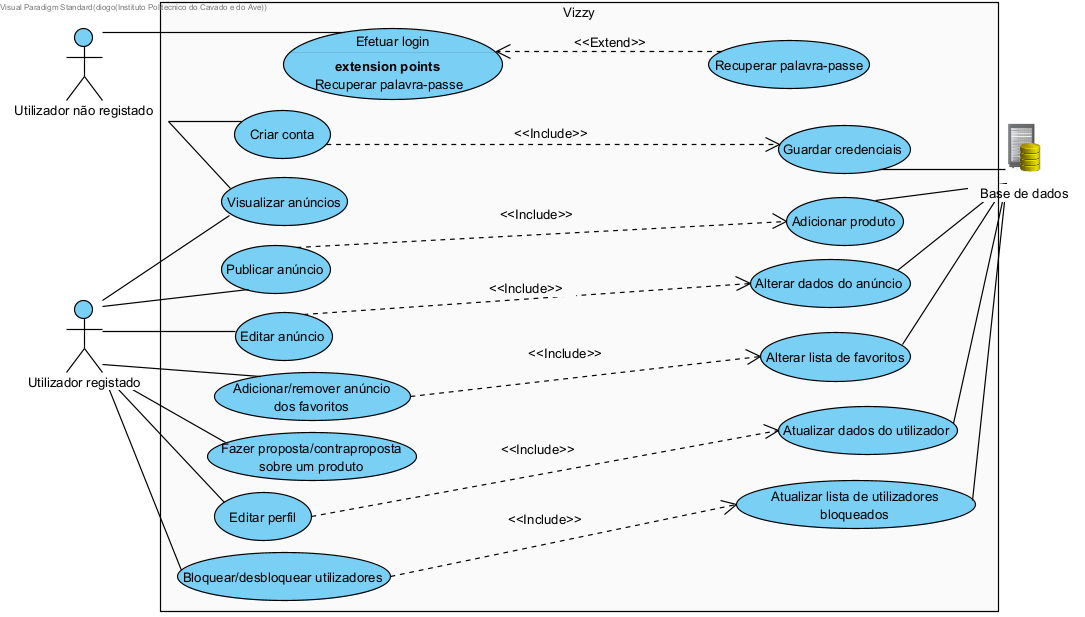
\includegraphics[width=\textwidth]{../images/use-case.png}
	\caption{Diagrama de casos de uso}
	\label{fig:casos de uso}
\end{figure}

O diagrama de casos de uso apresentado ilustra as principais interações dos utilizadores com o sistema \textit{Vizzy}. Existem dois tipos de utilizadores: \textbf{Utilizador não autenticado} e \textbf{Utilizador autenticado}, cada um com diferentes permissões e funcionalidades disponíveis.

\subsection{Utilizador Não Autenticado}
Os utilizadores que ainda não estão autenticados podem realizar as seguintes ações:
\begin{itemize}
	\item \textbf{Efetuar login} – Possibilidade de iniciar sessão no sistema. Este caso de uso pode ser estendido pela funcionalidade de \textbf{Recuperar palavra-passe}, caso o utilizador tenha perdido as credenciais de acesso.
	\item \textbf{Criar conta} – Processo de registo de novos utilizadores, que inclui a ação de \textbf{Guardar credenciais} na base de dados.
	\item \textbf{Visualizar anúncios} – Permite que os utilizadores não autenticados consultem os anúncios disponíveis.
\end{itemize}

\subsection{Utilizador Autenticados}
Após a autenticação, os utilizadores passam a ter acesso a funcionalidades adicionais, tais como:
\begin{itemize}
	\item \textbf{Publicar anúncio} – Possibilidade de adicionar um novo produto ao sistema. Este caso de uso inclui a funcionalidade de \textbf{Adicionar produto} à base de dados.
	\item \textbf{Editar anúncio} – Permite modificar um anúncio já publicado, incluindo a funcionalidade de \textbf{Alterar dados do anúncio}.
	\item \textbf{Adicionar/remover anúncio dos favoritos} – Possibilidade de gerir uma lista de favoritos, incluindo a ação de \textbf{Alterar lista de favoritos}.
	\item \textbf{Fazer proposta/contraproposta sobre um produto} – Funcionalidade que permite negociar produtos entre utilizadores autenticados.
	\item \textbf{Editar perfil} – Opção para alterar as informações da conta, incluindo a funcionalidade de \textbf{Atualizar dados do utilizador}.
	\item \textbf{Bloquear/desbloquear utilizadores} – Permite que um utilizador bloqueie ou desbloqueie outros, com a ação correspondente de \textbf{Atualizar lista de utilizadores bloqueados} na base de dados.
\end{itemize}

O diagrama demonstra as relações entre os casos de uso através de conexões do tipo \textbf{include} (\texttt{<<include>>}) e \textbf{extend} (\texttt{<<extend>>}), assegurando que determinadas ações dependem de outras funcionalidades do sistema. Além disso, todas as operações que envolvem a manipulação de dados refletem diretamente na \textbf{Base de Dados}, que armazena e gere as informações essenciais para o funcionamento da plataforma.
%------------------------------------------------
\newpage
\section{Diagramas BPMN}

Os \textbf{diagramas BPMN} (\textit{Business Process Model and Notation}) são uma forma padronizada de representar visualmente processos de negócio. Eles utilizam símbolos gráficos para descrever o fluxo de atividades, decisões e interações dentro de uma aplicação, facilitando a compreensão e a análise dos processos de negócio.

\subsection{Diagrama BPMN das vendas}

\begin{figure}[ht]
	\centering
	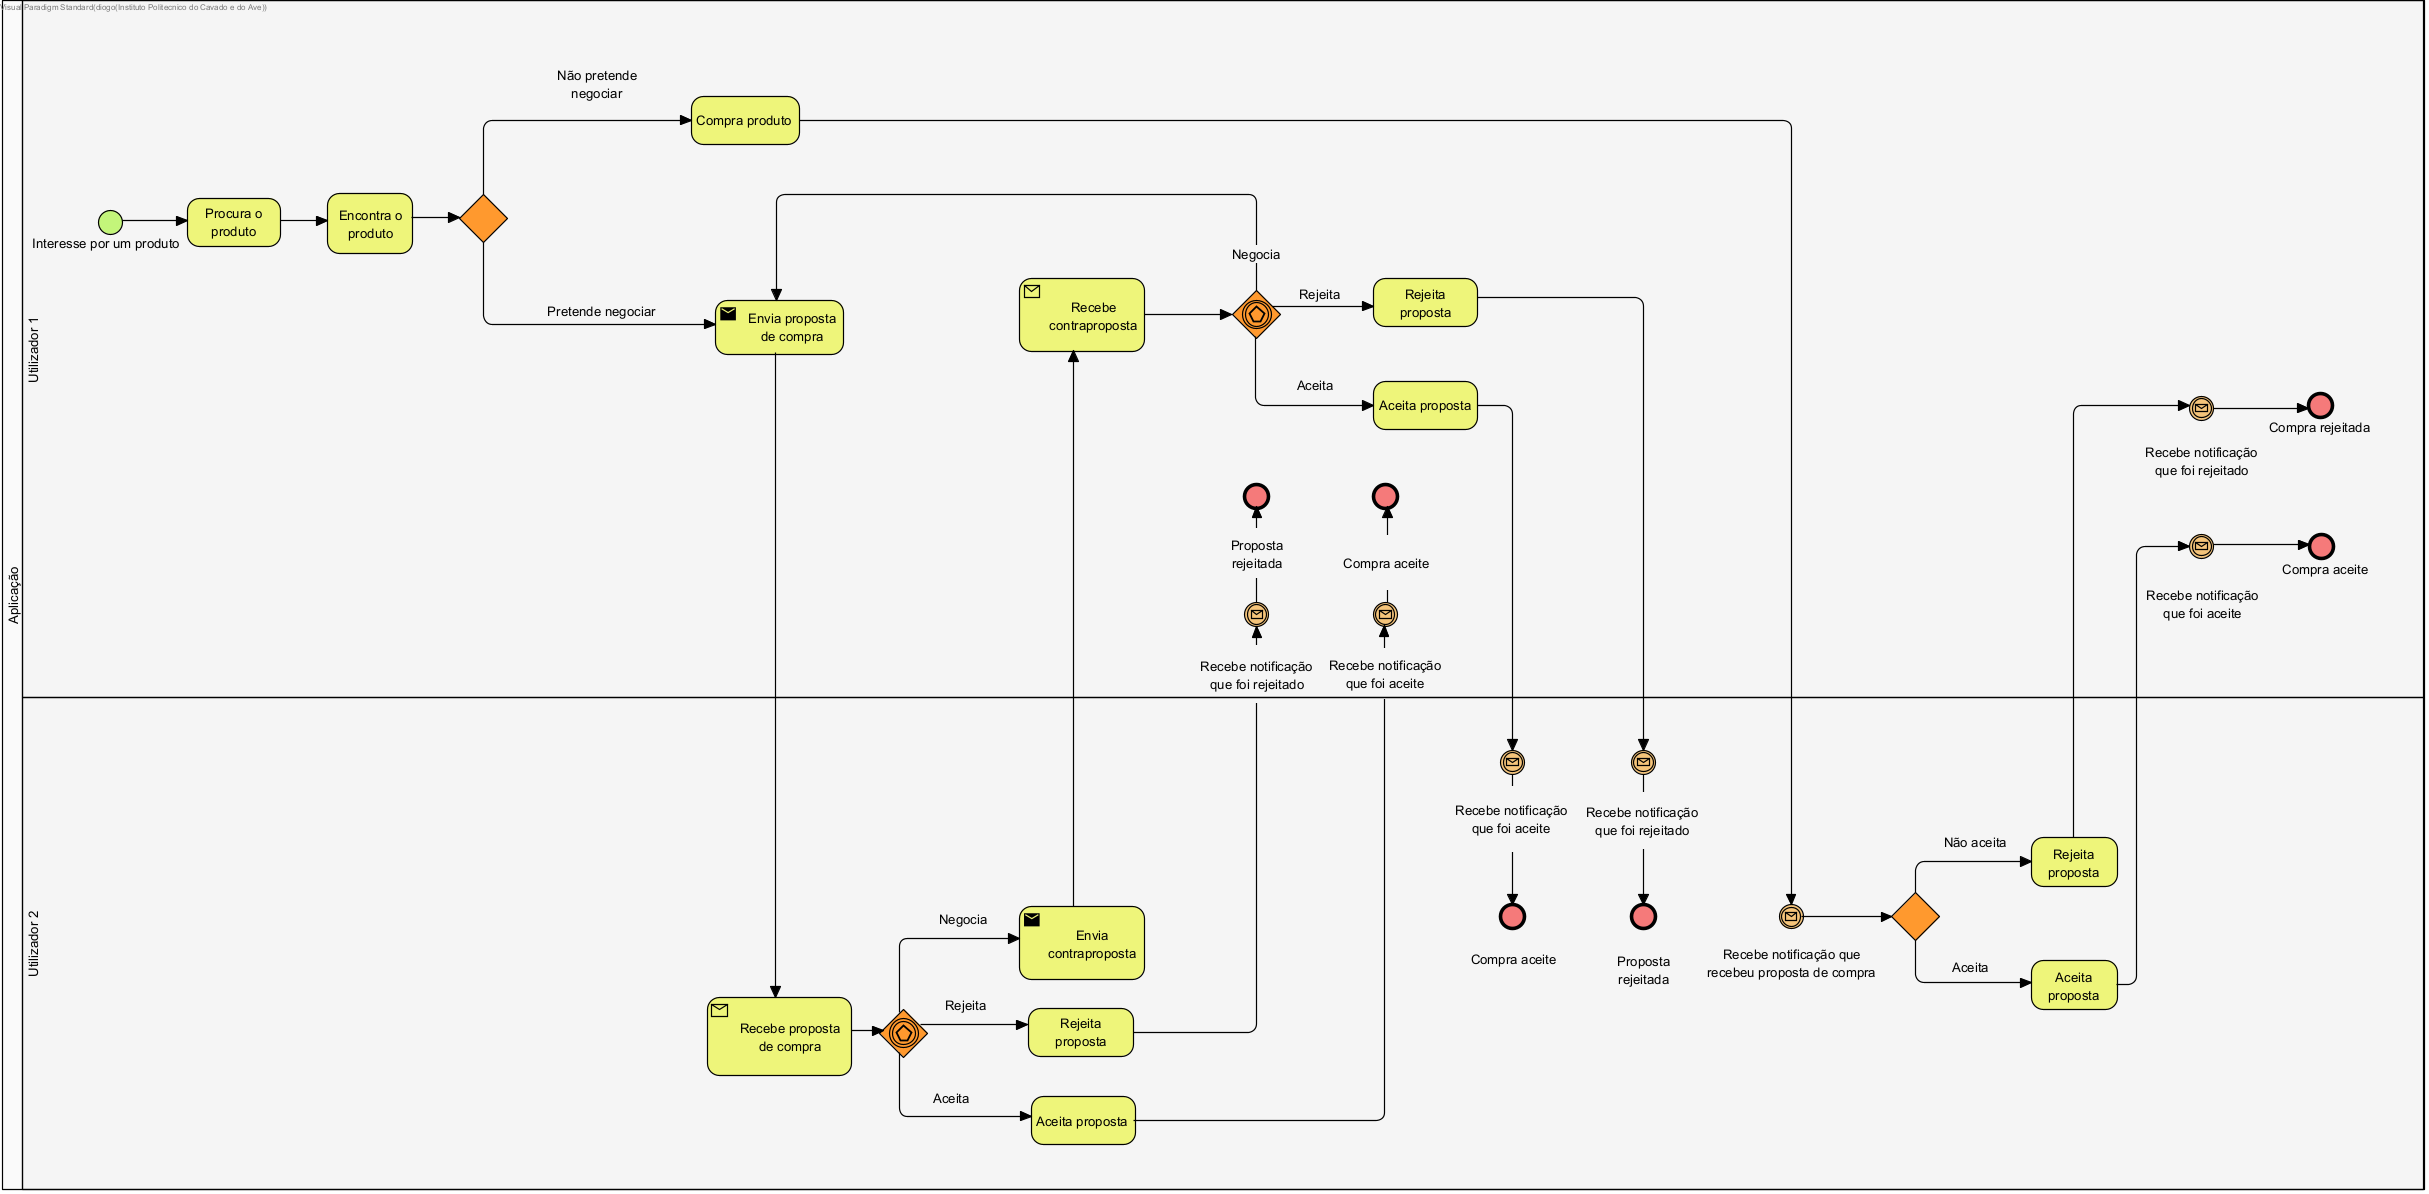
\includegraphics[width=\textwidth]{../images/bpmn-sales.png}
	\caption{Diagrama BPMN das vendas}
	\label{fig:bpmn vendas}
\end{figure}


O diagrama BPMN apresentado representa o processo de negociação e compra de um produto entre dois utilizadores. O fluxo de atividades está dividido em duas \textit{pools} , correspondendo ao \textbf{Utilizador 1} e ao \textbf{Utilizador 2}, cada um desempenhando diferentes papéis dentro do processo.

O processo inicia-se quando o \textbf{Utilizador 1} demonstra \textbf{interesse por um produto}. A partir deste ponto, segue-se o seguinte fluxo:

\begin{itemize}
	\item O \textbf{Utilizador 1} realiza a \textbf{procura pelo produto} e, ao encontrá-lo, decide se pretende negociar ou comprá-lo diretamente.
	\item Se optar por \textbf{não negociar}, procede à \textbf{compra do produto}.
	\item Caso opte por negociar, envia uma \textbf{proposta de compra} ao \textbf{Utilizador 2}.
	\item O \textbf{Utilizador 2} pode:
	\begin{itemize}
		\item \textbf{Aceitar a proposta}, finalizando a compra.
		\item \textbf{Rejeitar a proposta}, encerrando a negociação.
		\item \textbf{Enviar uma contraproposta}, iniciando um ciclo de negociação.
	\end{itemize}
	\item Se o \textbf{Utilizador 1} receber uma contraproposta, pode novamente decidir entre aceitá-la, rejeitá-la ou enviar uma nova proposta.
\end{itemize}


O processo pode resultar em dois desfechos:
\begin{itemize}
	\item \textbf{Compra aceite}: Quando uma das partes aceita a proposta ou contraproposta.
	\item \textbf{Compra rejeitada}: Se uma das partes rejeitar a proposta.
\end{itemize}

\subsection{Diagrama BPMN dos empréstimos/alugueres}

\begin{figure}[ht]
	\centering
	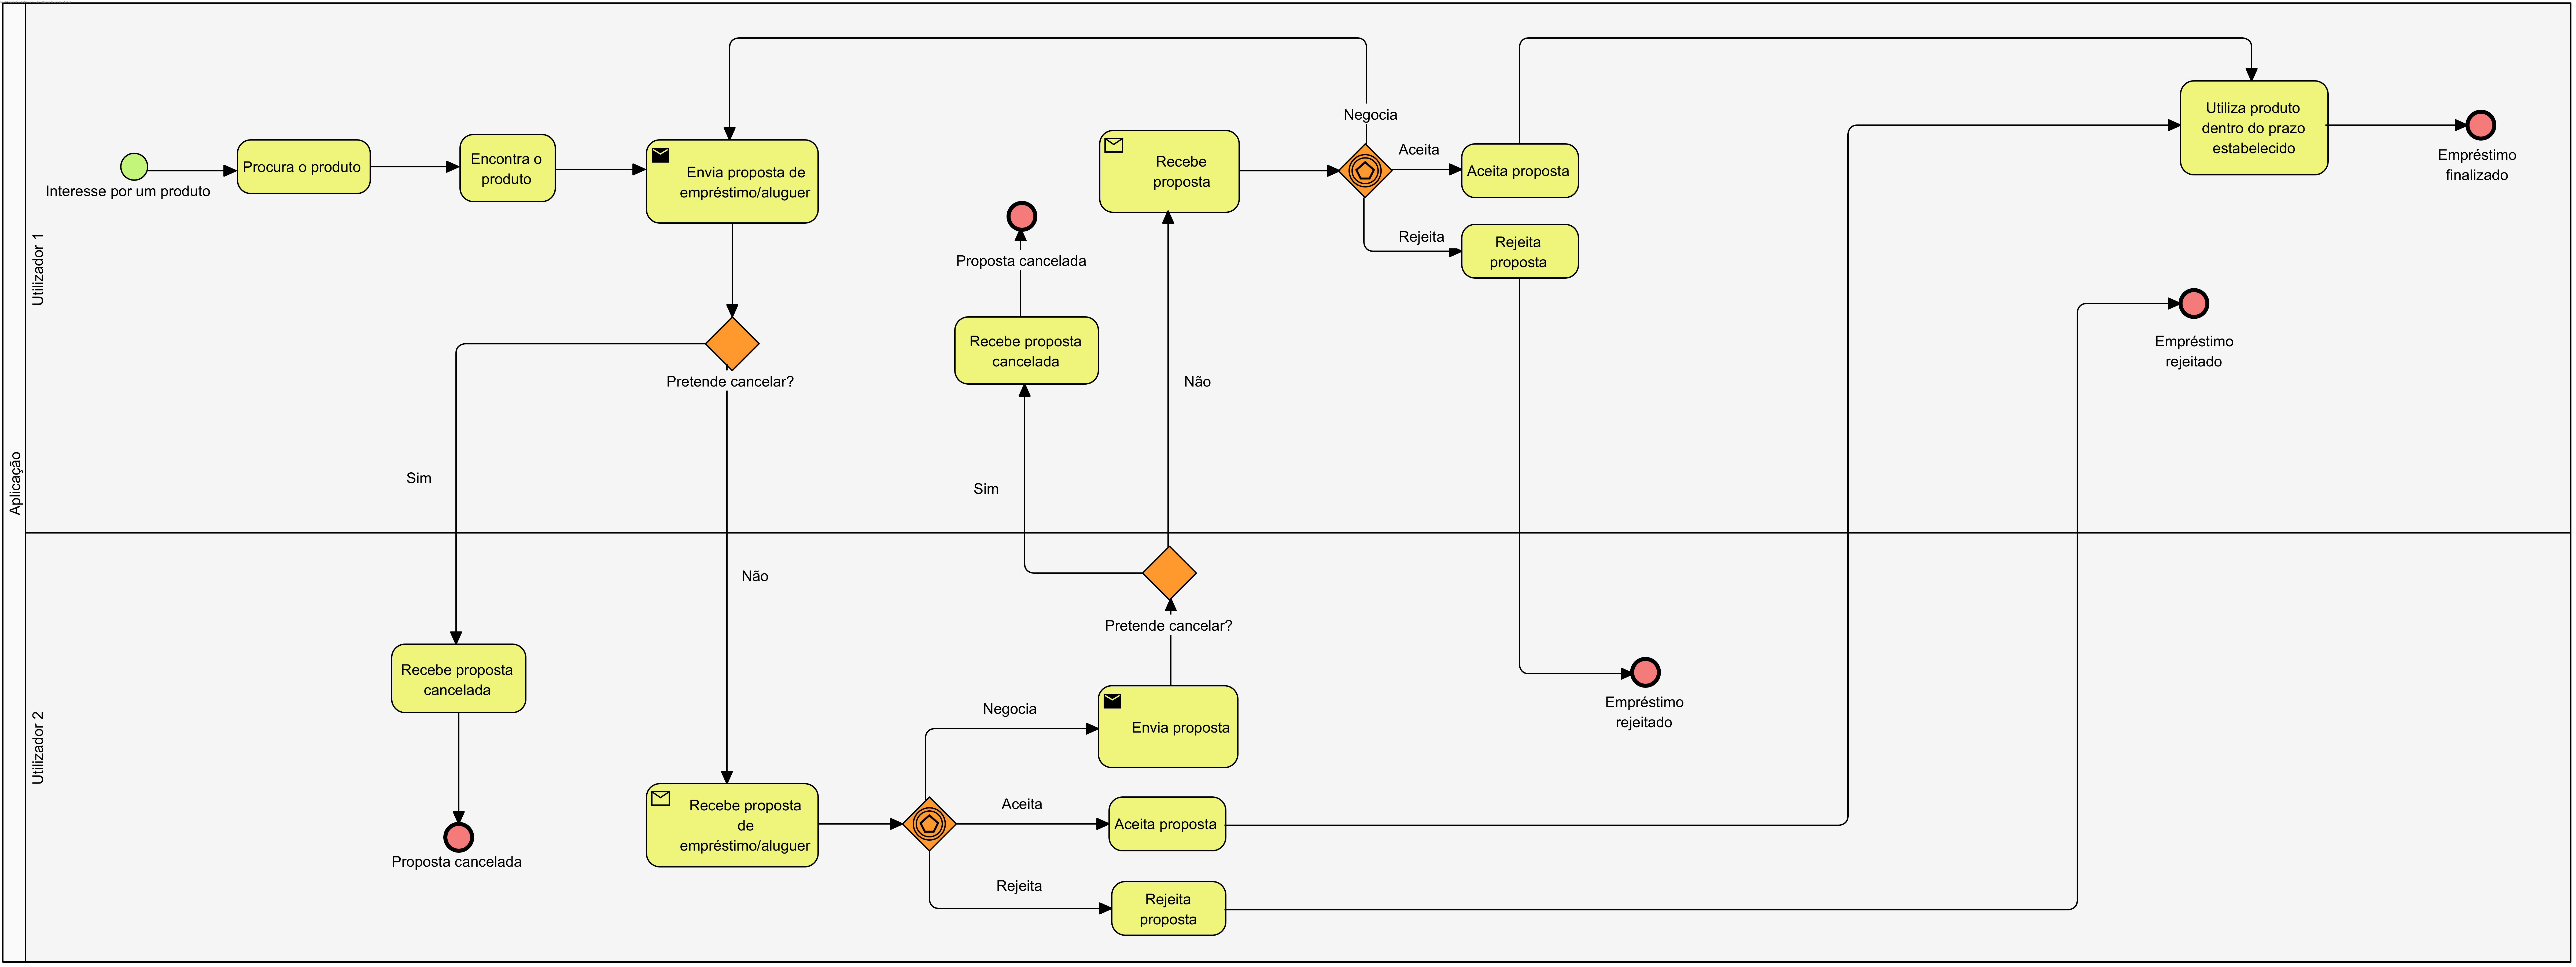
\includegraphics[width=\textwidth]{../images/bpmn-rentals.png}
	\caption{Diagrama BPMN dos empréstimos/alugueres}
	\label{fig:bpmn emprestimo/aluguer}
\end{figure}

O diagrama BPMN apresentado representa o processo de negociação de empréstimo/aluguer de um produto entre dois utilizadores. O fluxo de atividades está dividido em duas \textit{pools}, correspondendo ao \textbf{Utilizador 1} e ao \textbf{Utilizador 2}, cada um desempenhando diferentes papéis dentro do processo. O processo inicia-se quando o \textbf{Utilizador 1} demonstra \textbf{interesse por um produto}. A partir deste ponto, segue-se o seguinte fluxo:

\begin{itemize}
	\item O \textbf{Utilizador 1} realiza a \textbf{procura pelo produto} na aplicação.
	\item Após encontrar o produto, envia uma \textbf{proposta de empréstimo/aluguer} ao \textbf{Utilizador 2}.
	\item O \textbf{Utilizador 2} pode:
	\begin{itemize}
		\item \textbf{Aceitar a proposta}, iniciando o processo de empréstimo.
		\item \textbf{Rejeitar a proposta}, encerrando a negociação.
		\item \textbf{Enviar uma contraproposta}, iniciando um ciclo de negociação.
	\end{itemize}
	\item Se o \textbf{Utilizador 1} receber uma contraproposta, pode novamente decidir entre aceitá-la, rejeitá-la ou enviar uma nova proposta.
\end{itemize}

O processo pode resultar em dois desfechos:
\begin{itemize}
	\item \textbf{Empréstimo aceite}: Quando uma das partes aceita a proposta ou contraproposta. O produto é utilizado dentro do prazo estabelecido e depois devolvido.
	\item \textbf{Empréstimo rejeitado}: Se uma das partes rejeitar a proposta, o processo é encerrado.
\end{itemize}

Após a devolução do produto, o \textbf{Utilizador 2} confirma a sua receção, concluindo o processo de empréstimo.

\newpage
\subsection{Diagrama BPMN das trocas}

\begin{figure}[ht]
	\centering
	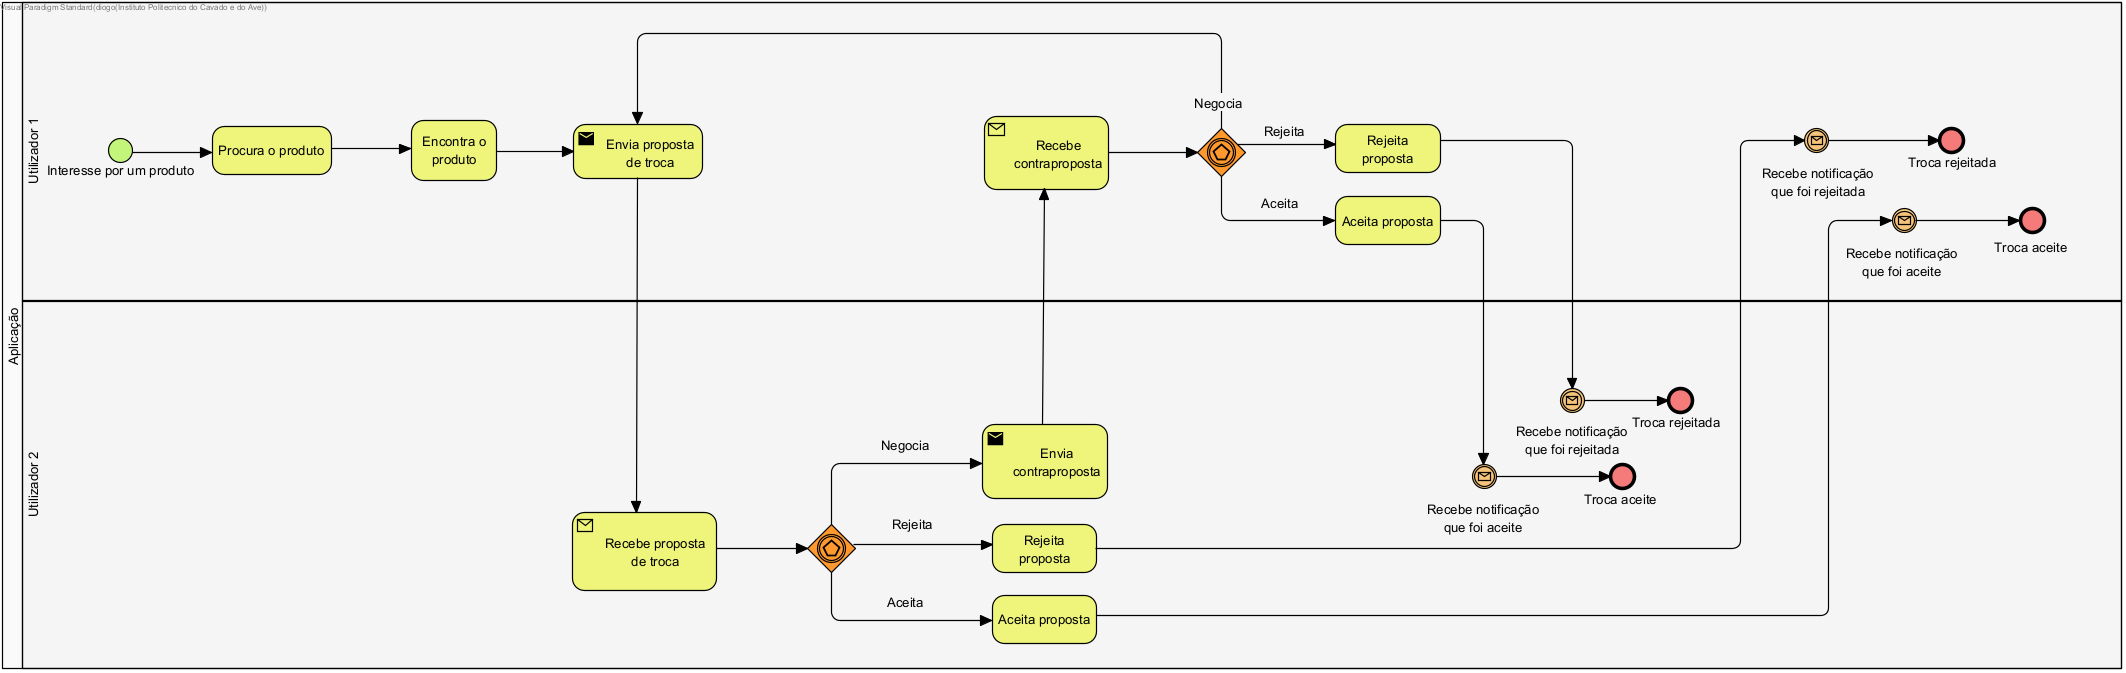
\includegraphics[width=\textwidth]{../images/bpmn-swaps.png}
	\caption{Diagrama BPMN das trocas}
	\label{fig:bpmn trocas}
\end{figure}

O diagrama BPMN apresentado descreve o processo de negociação e troca de produtos entre dois utilizadores. O fluxo está dividido em duas \textit{pools}, representando o \textbf{Utilizador 1} e o \textbf{Utilizador 2}, cada um com diferentes papéis no processo. O processo inicia-se quando o \textbf{Utilizador 1} demonstra \textbf{interesse por um produto}. O fluxo de atividades segue a seguinte sequência:

\begin{itemize}
	\item O \textbf{Utilizador 1} procura um produto e envia uma \textbf{proposta de troca} ao \textbf{Utilizador 2}.
	\item O \textbf{Utilizador 2} pode:
	\begin{itemize}
		\item \textbf{Aceitar a proposta}, finalizando a troca.
		\item \textbf{Rejeitar a proposta}, encerrando a negociação.
		\item \textbf{Enviar uma contraproposta}, iniciando um ciclo de negociação.
	\end{itemize}
	\item Se o \textbf{Utilizador 1} receber uma contraproposta, pode decidir entre aceitá-la, rejeitá-la ou enviar uma nova proposta.
\end{itemize}

O processo pode resultar em dois desfechos:
\begin{itemize}
	\item \textbf{Troca aceite}: Quando uma das partes aceita a proposta ou contraproposta.
	\item \textbf{Troca rejeitada}: Se uma das partes rejeitar a proposta.
\end{itemize}
%------------------------------------------------
\newpage
\section{Diagrama ER}

O diagrama representa um sistema onde os utilizadores podem comprar, vender, alugar ou trocar produtos. A estrutura do modelo de dados é composta por várias tabelas interligadas, refletindo diferentes tipos de anúncio, propostas e transações.



\subsection{\textbf{Utilizadores (users)}}
Os utilizadores terão como dados um \textit{username}, um email e o seu nome. Para além disso terão números de contacto e uma localização associados e também uma lista de utilizadores bloqueados e de anúncios favoritos.



\subsection{\textbf{Principais Tabelas e Relações}}

\subsubsection{\textbf{Utilizadores (users)}}

\begin{itemize}
	\item Contém informações dos utilizadores, como nome, email e localização.
	\item Campos importantes:
	\begin{itemize}
		\item \verb|id| (UUID): Identificador único do utilizador.
		\item \verb|username|, \verb|email|, \verb|name|: Dados pessoais.
		\item \verb|location_id|: Referência à localização do utilizador.
		\item \verb|is_deleted|, \verb|deleted_at|: Indicam se a conta foi apagada.
	\end{itemize}
	\item Ligações:
	\begin{itemize}
		\item \textbf{locations} (cidade e país do utilizador).
		\item \textbf{blocked\_users} (gestão de bloqueios entre utilizadores).
		\item \textbf{favorites} (anúncios favoritos do utilizador).
		\item \textbf{contacts} (dados de contacto do utilizador).
		\item \textbf{user\_transactions} (associação com transações).
	\end{itemize}
\end{itemize}

\subsubsection{\textbf{Listagens de Produtos (product\_listings)}}

\begin{itemize}
	\item Representa os produtos anunciados pelos utilizadores.
	\item Campos importantes:
	\begin{itemize}
		\item \verb|id|: Identificador único do anúncio.
		\item \verb|title|, \verb|description|: Informações do item.
		\item \verb|date_created|: Data de criação do anúncio.
		\item \verb|owner_id|: Utilizador que criou o anúncio.
		\item \verb|category_id|: Categoria do produto.
		\item \verb|listing_status|: Estado do anúncio.
	\end{itemize}
	\item Ligações:
	\begin{itemize}
		\item \textbf{listing\_statuses} (estado do anúncio: ativo, expirado, etc.).
		\item \textbf{product\_categories} (categoria do produto).
		\item \textbf{product\_images} (imagens associadas ao produto).
		\item Diferentes tipos de anúncios: \textbf{sale\_listings}, \textbf{rental\_listings}, \textbf{swap\_listings} e \textbf{giveaway\_listings}.
	\end{itemize}
\end{itemize}

\subsubsection{\textbf{Tipos de Anúncios}}

\begin{itemize}
	\item \textbf{sale\_listings}: Inclui preço, condição do produto e se o preço é negociável.
	\item \textbf{rental\_listings}: Contém dados como custo diário, depósito e limite de duração do aluguer.
	\item \textbf{swap\_listings}: Define o item desejado para troca.
	\item \textbf{giveaway\_listings}: Especifica requisitos para doação do item.
\end{itemize}

\subsubsection{\textbf{Propostas (proposals)}}

\begin{itemize}
	\item Regista propostas de transação entre utilizadores.
	\item Campos principais:
	\begin{itemize}
		\item \verb|id|: Identificador único.
		\item \verb|sender_id|, \verb|receiver_id|: Utilizadores envolvidos.
		\item \verb|listing_id|: Produto associado à proposta.
		\item \verb|proposal_type_id|: Tipo de proposta (troca, venda, aluguer, doação).
		\item \verb|proposal_status_id|: Estado da proposta.
	\end{itemize}
	\item Ligações:
	\begin{itemize}
		\item \textbf{proposal\_types} (tipo de proposta).
		\item \textbf{proposal\_statuses} (estado da proposta).
		\item \textbf{proposal\_images} (imagens associadas às propostas).
		\item Tipos específicos de propostas:
		\begin{itemize}
			\item \textbf{sale\_proposals} (inclui preço oferecido).
			\item \textbf{rental\_proposals} (informações de aluguer).
			\item \textbf{swap\_proposals} (itens de troca).
			\item \textbf{giveaway\_proposals} (mensagem para doação).
		\end{itemize}
	\end{itemize}
\end{itemize}

\subsubsection{\textbf{Transações (transactions)}}

\begin{itemize}
	\item Armazena transações concluídas na plataforma.
	\item Campos principais:
	\begin{itemize}
		\item \verb|id|: Identificador único.
		\item \verb|date_created|: Data da transação.
		\item \verb|transaction_status_id|: Estado da transação.
		\item \verb|listing_id|: Produto transacionado.
		\item \verb|proposal_id|: Proposta que originou a transação.
		\item \verb|user_id|: Utilizador envolvido.
	\end{itemize}
	\item Ligações:
	\begin{itemize}
		\item \textbf{transaction\_statuses} (estado da transação).
		\item \textbf{user\_transactions} (relação entre comprador e vendedor).
	\end{itemize}
\end{itemize}

\subsubsection{\textbf{Outras tabelas de suporte}}

\begin{itemize}
	\item \textbf{locations}: Armazena informações sobre a localização do utilizador.
	\item \textbf{contacts}: Regista detalhes de contacto.
	\item \textbf{favorites}: Guarda anúncios marcados como favoritos pelos utilizadores.
	\item \textbf{blocked\_users}: Relação entre utilizadores bloqueados.
	\item \textbf{product\_categories}: Define as categorias dos produtos.
	\item \textbf{product\_images}: Associa imagens aos anúncios.
	\item \textbf{rental\_availabilities}: Especifica a disponibilidade de aluguer.
\end{itemize}

\begin{figure}[ht]
	\centering
	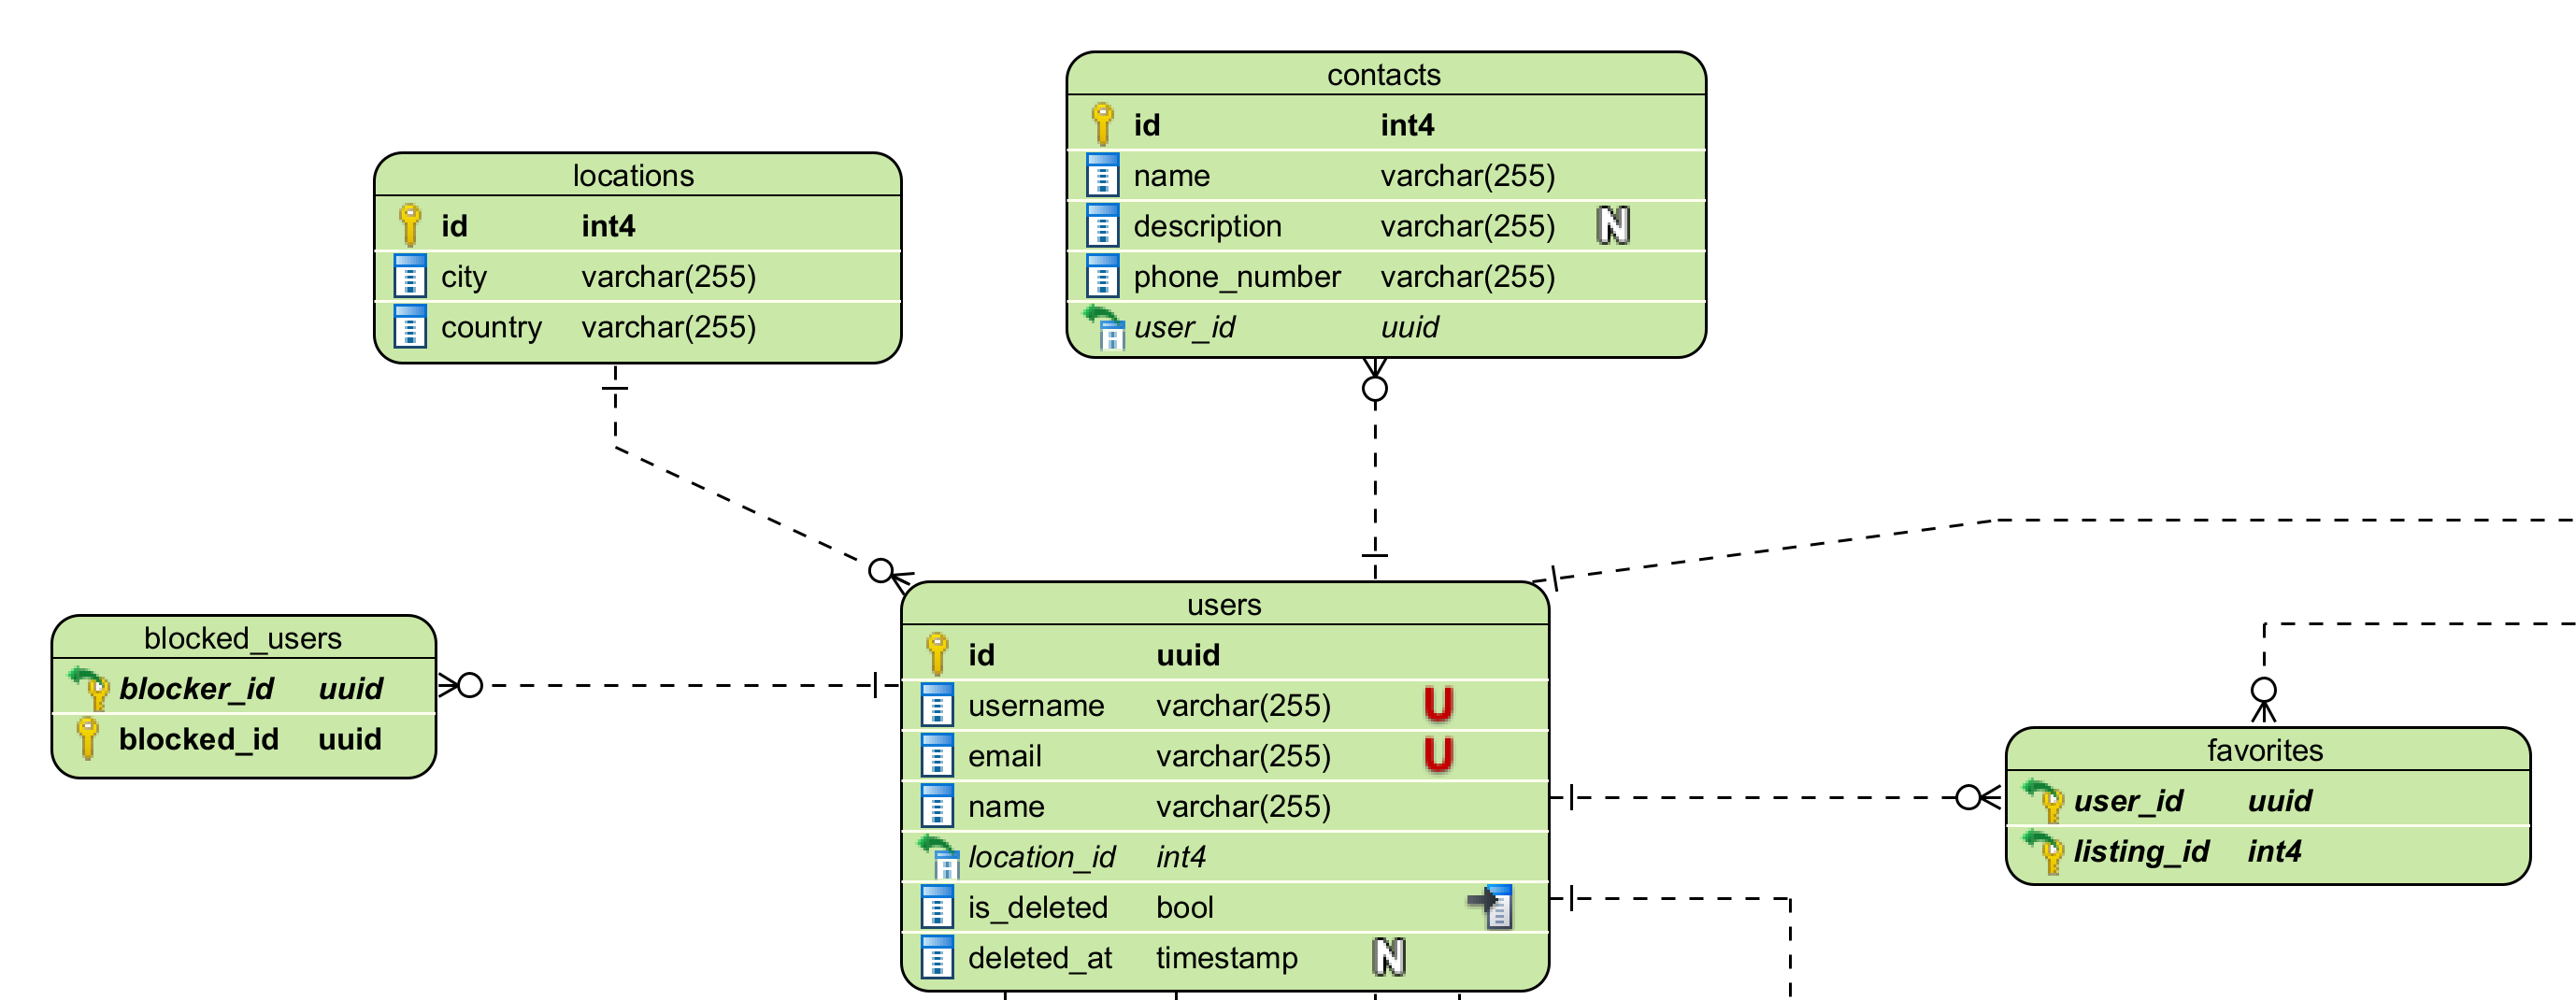
\includegraphics[width=\textwidth]{../images/entity-relationship-diagram-users.png}
	\caption{Diagrama ER - Utilizadores}
	\label{fig:ER Users}
\end{figure}
\newpage
\subsection{\textbf{Anúncios de Produtos (product\_listings)}}

A tabela de \textbf{\textit{product\_listing}} terá os atributos que serão comuns a todos os tipos de anúncios como o titulo, a descrição e a data que foi criado, mas depois irão existir três tipo de produtos:

\begin{itemize}
	\item \textbf{sale\_listing} - Anúncios para venda, com preço e condição do produto.
	\item \textbf{swap\_listing} - Anúncios de troca.
	\item \textbf{giveaway\_listing} - Anúncios de oferta gratuita, com requisitos opcionais.
	\item \textbf{rental\_listing} - Anúncios de aluguer, incluindo caução e preços.
\end{itemize}
Num anúncio também poderão estar associados imagens do produto e a sua categoria. Para além disso também teremos o estado do anúncio.
\begin{figure}[H]
	\centering
	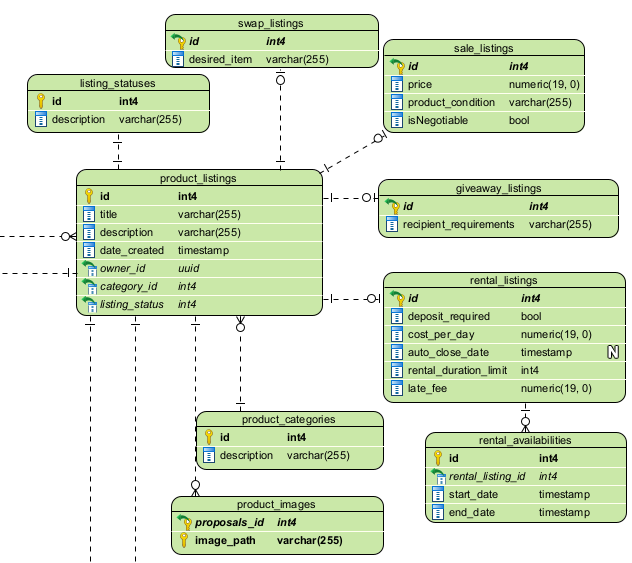
\includegraphics[width=\textwidth, height=10cm]{../images/entity-relationship-diagram-listings.png}
	\caption{Diagrama ER - Anúncios}
	\label{fig:ER Listings}
\end{figure}

\newpage

\subsection{\textbf{Propostas (proposals)}}
A tabela de \textbf{\textit{proposals}} contém mais uma vez os atributos que são comuns a todo o tipo de propostas que são o titulo e a descrição. Depois teremos tabelas para cada tipo de proposta que são:


\begin{itemize}
	\item \textbf{swap\_proposal} - Propostas de troca de produtos.
	\item \textbf{sale\_proposal} - Propostas de venda, com um preço proposto.
	\item \textbf{giveaway\_proposal} - Propostas de oferta sem custo.
	\item \textbf{rental\_proposal} - Propostas de aluguer, incluindo datas de início e fim.
\end{itemize}

Para além disso também teremos uma tabela com o estado da proposta
\begin{figure}[H]
	\centering
	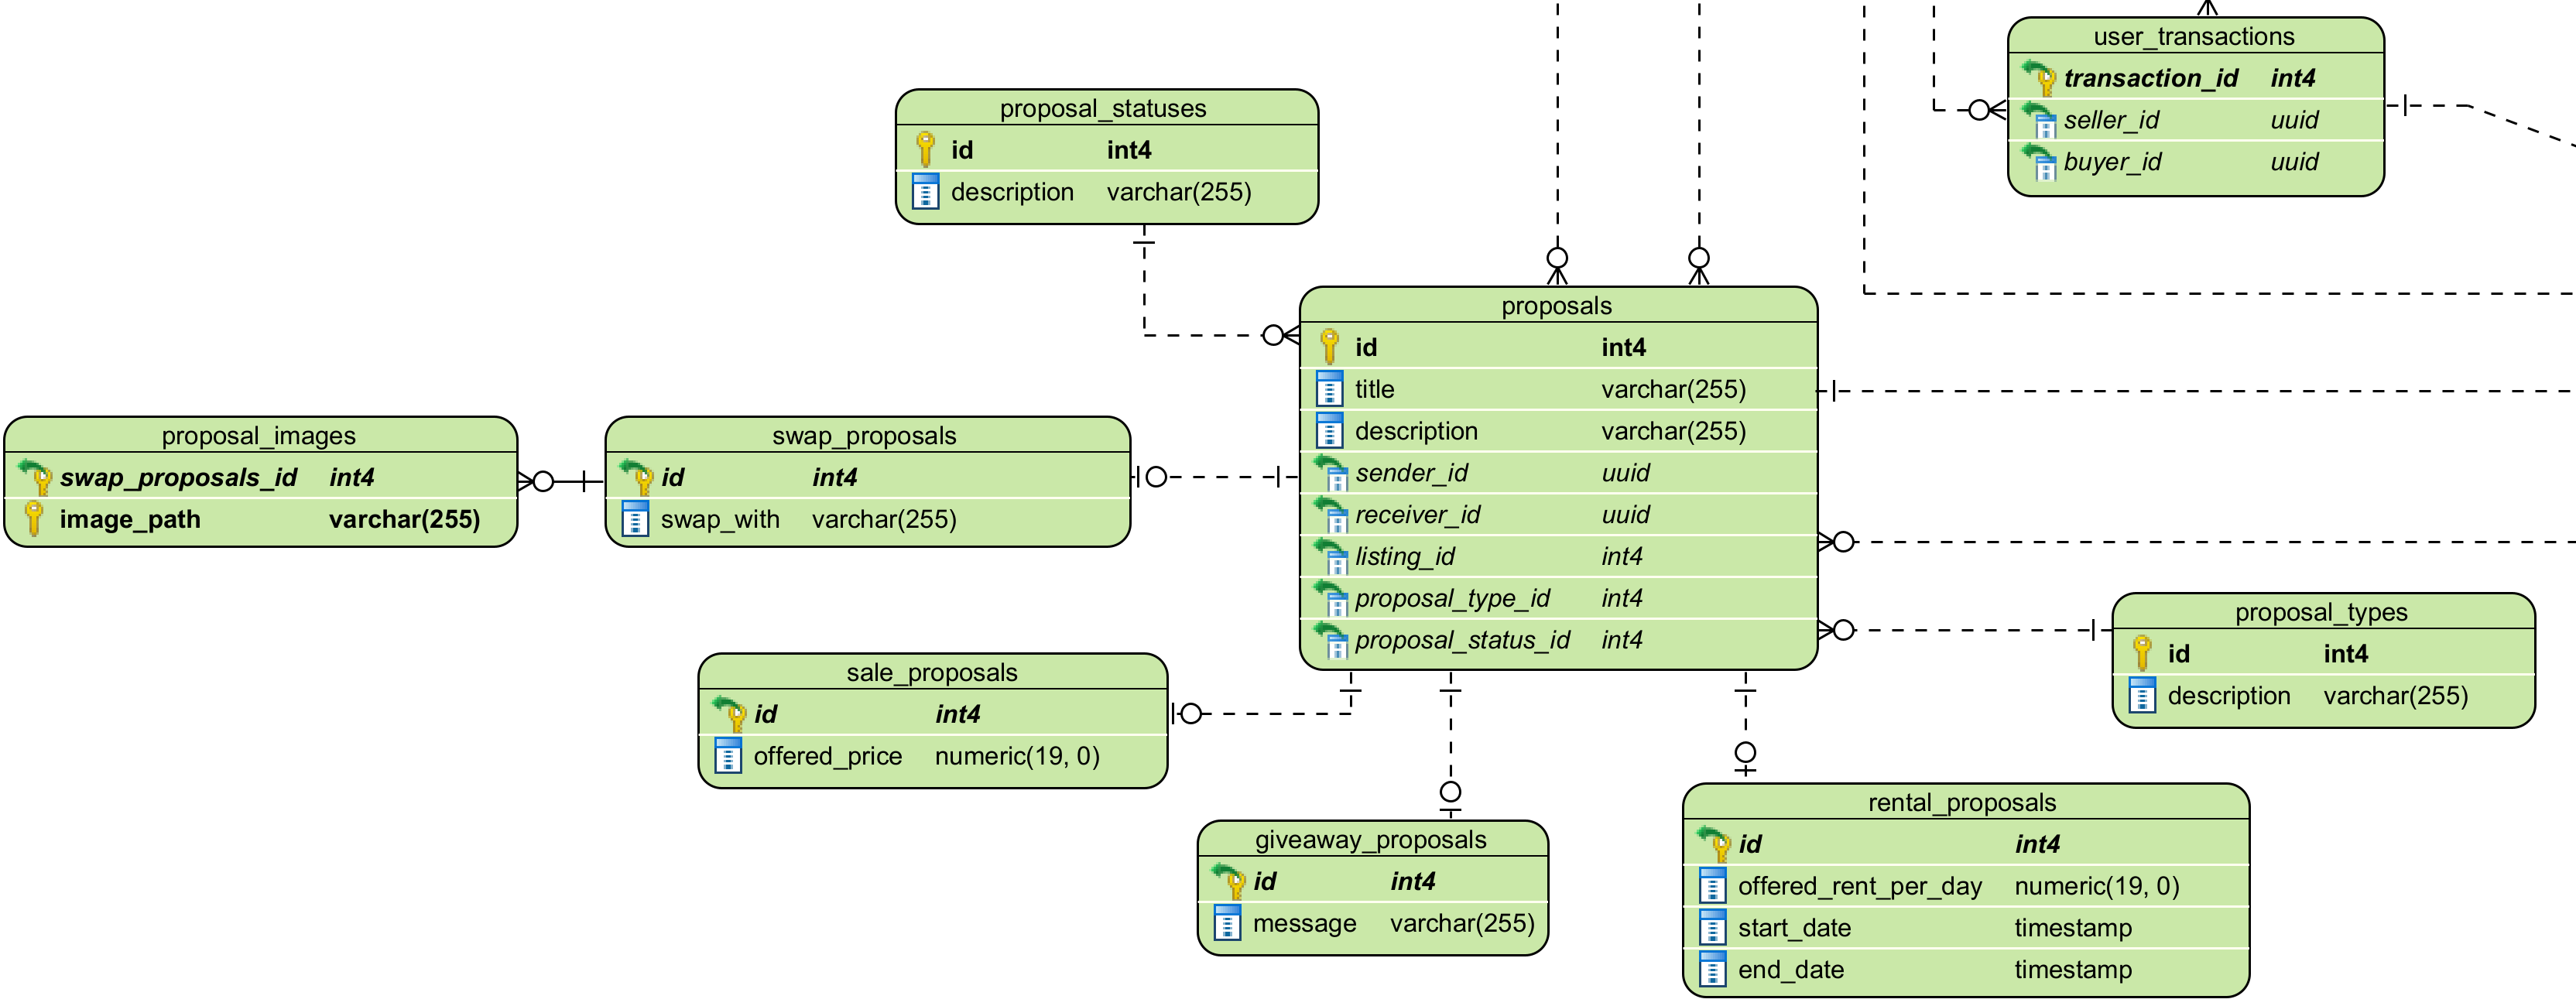
\includegraphics[width=\textwidth]{../images/entity-relationship-diagram-proposals.png}
	\caption{Diagrama ER - Propostas}
	\label{fig:ER Proposals}
\end{figure}

\newpage

\subsection{\textbf{Transações (transactions)}}
Na tabela \textbf{\textit{transactions}} temos a data que essa transação foi criada e uma associação a uma tabela com o estado dessa mesma transação. Para além disso também temos uma tabela \textbf{\textit{user\_transactions}} que terá como função servir de tabela intermediária que terá o \textbf{id} do comprador e do vendedor. 
\begin{figure}[H]
	\centering
	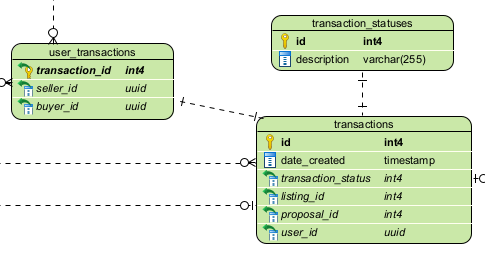
\includegraphics[width=\textwidth]{../images/entity-relationship-diagram-transactions.png}
	\caption{Diagrama ER - Transações}
	\label{fig:diagrama_er}
\end{figure}

%------------------------------------------------------------------------------------

\clearpage
\newpage
\section{Diagrama de Classes}

A API backend foi estruturada com modelos e controladores, organizados em pacotes como \textit{User Management}, \textit{Proposals}, \textit{Transactions} e \textit{Product Listings}. Cada pacote define classes com atributos e relações, que garante modularidade e escalabilidade.

\subsection{User Management}
O pacote \textit{User Management} gere as entidades relacionadas com utilizadores e as suas interações. A classe \textbf{User} armazena diversas informações, como \verb*|ID|, \verb*|nome|, \verb*|localização|, \verb*|contactos| e outros dados relevantes. Os utilizadores podem bloquear outros utilizadores (\textbf{BlockedUser}) e adicionar anúncios aos favoritos (\textbf{Favorite}).

\begin{figure}[ht]
	\centering
	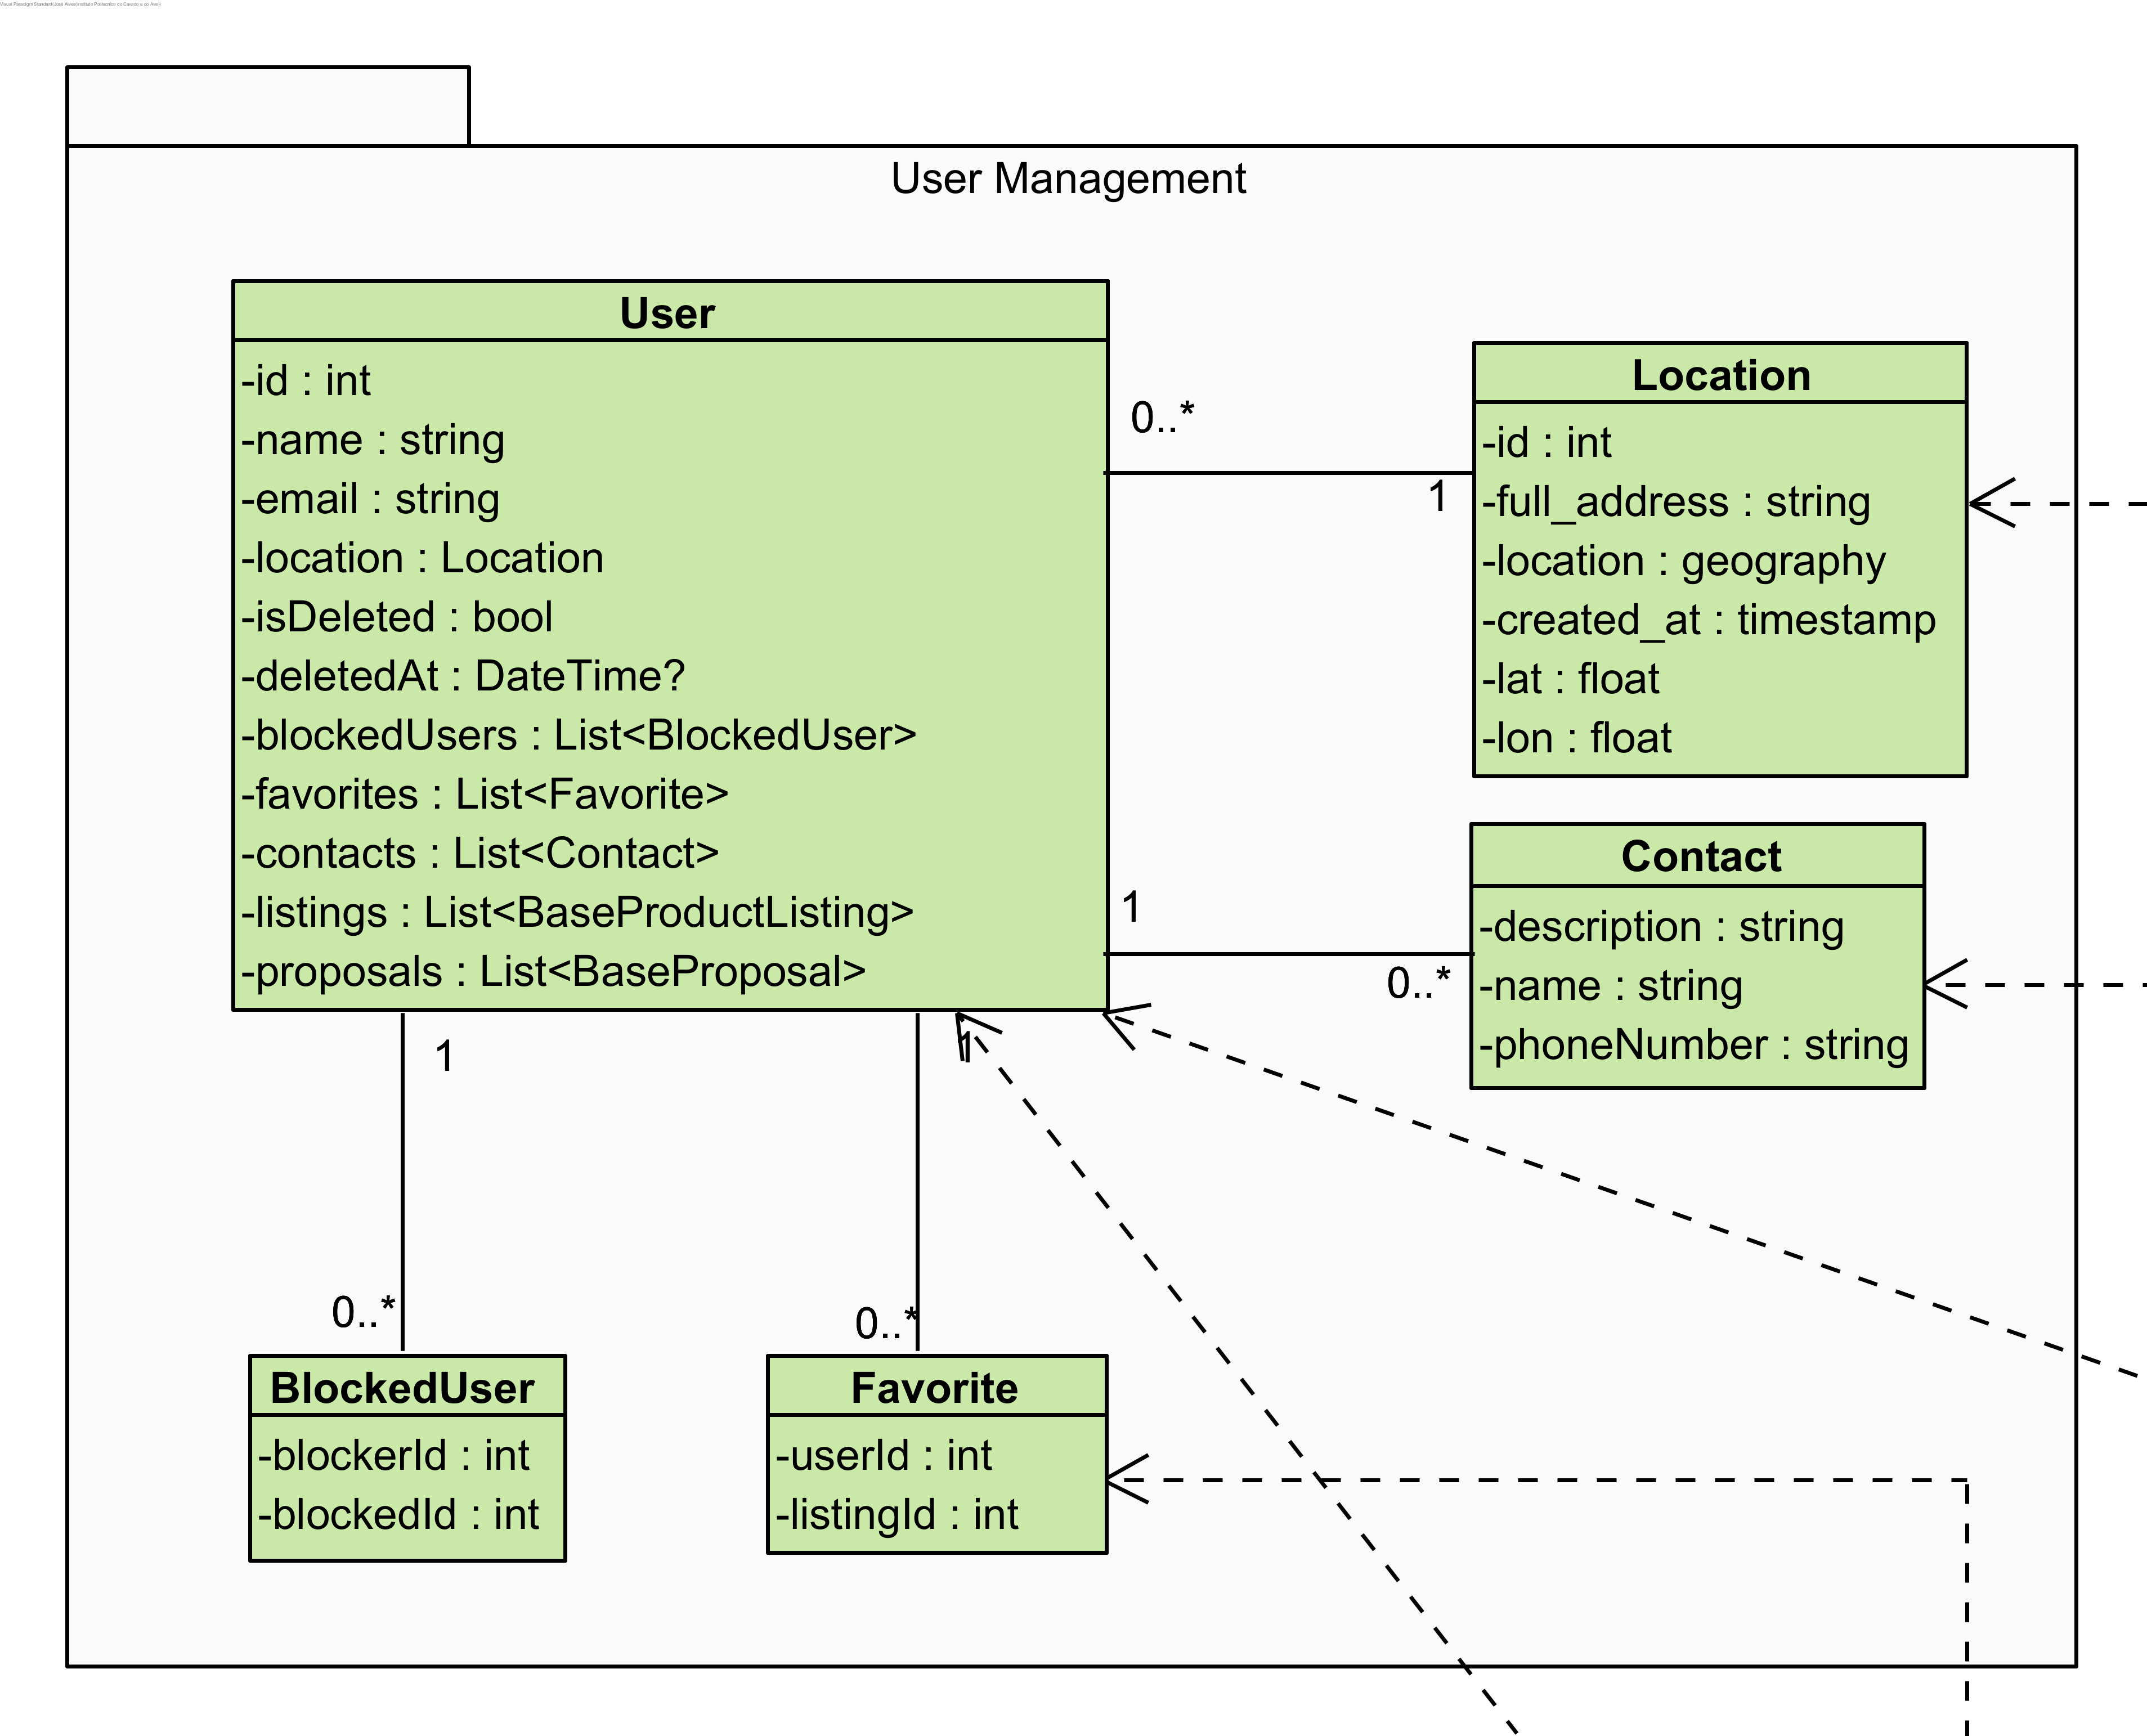
\includegraphics[width=\textwidth]{../images/class-diagram-user-management.png}
	\caption{Diagrama de Classes - Utilizadores}
	\label{fig:class_diagram_user_management}
\end{figure}

\subsection{Proposals}
O pacote \textit{Proposals} define os diferentes tipos de propostas que os utilizadores podem criar. A classe base \textbf{BaseProposal} contém atributos comuns a todas as propostas, como descrição, estado e utilizador associado. Tipos específicos incluem:
\begin{itemize}
	\item \textbf{SwapProposal} - Propostas de troca de produtos.
	\item \textbf{SaleProposal} - Propostas de venda, com um preço proposto.
	\item \textbf{GiveawayProposal} - Propostas de oferta sem custo.
	\item \textbf{RentalProposal} - Propostas de aluguer, incluindo datas de início e fim.
\end{itemize}
A classe \textbf{ProposalStatus} guarda o estado de uma proposta.

Propostas do tipo \textbf{SwapProposal} (troca) têm imagens associadas.

\begin{figure}[ht]
	\centering
	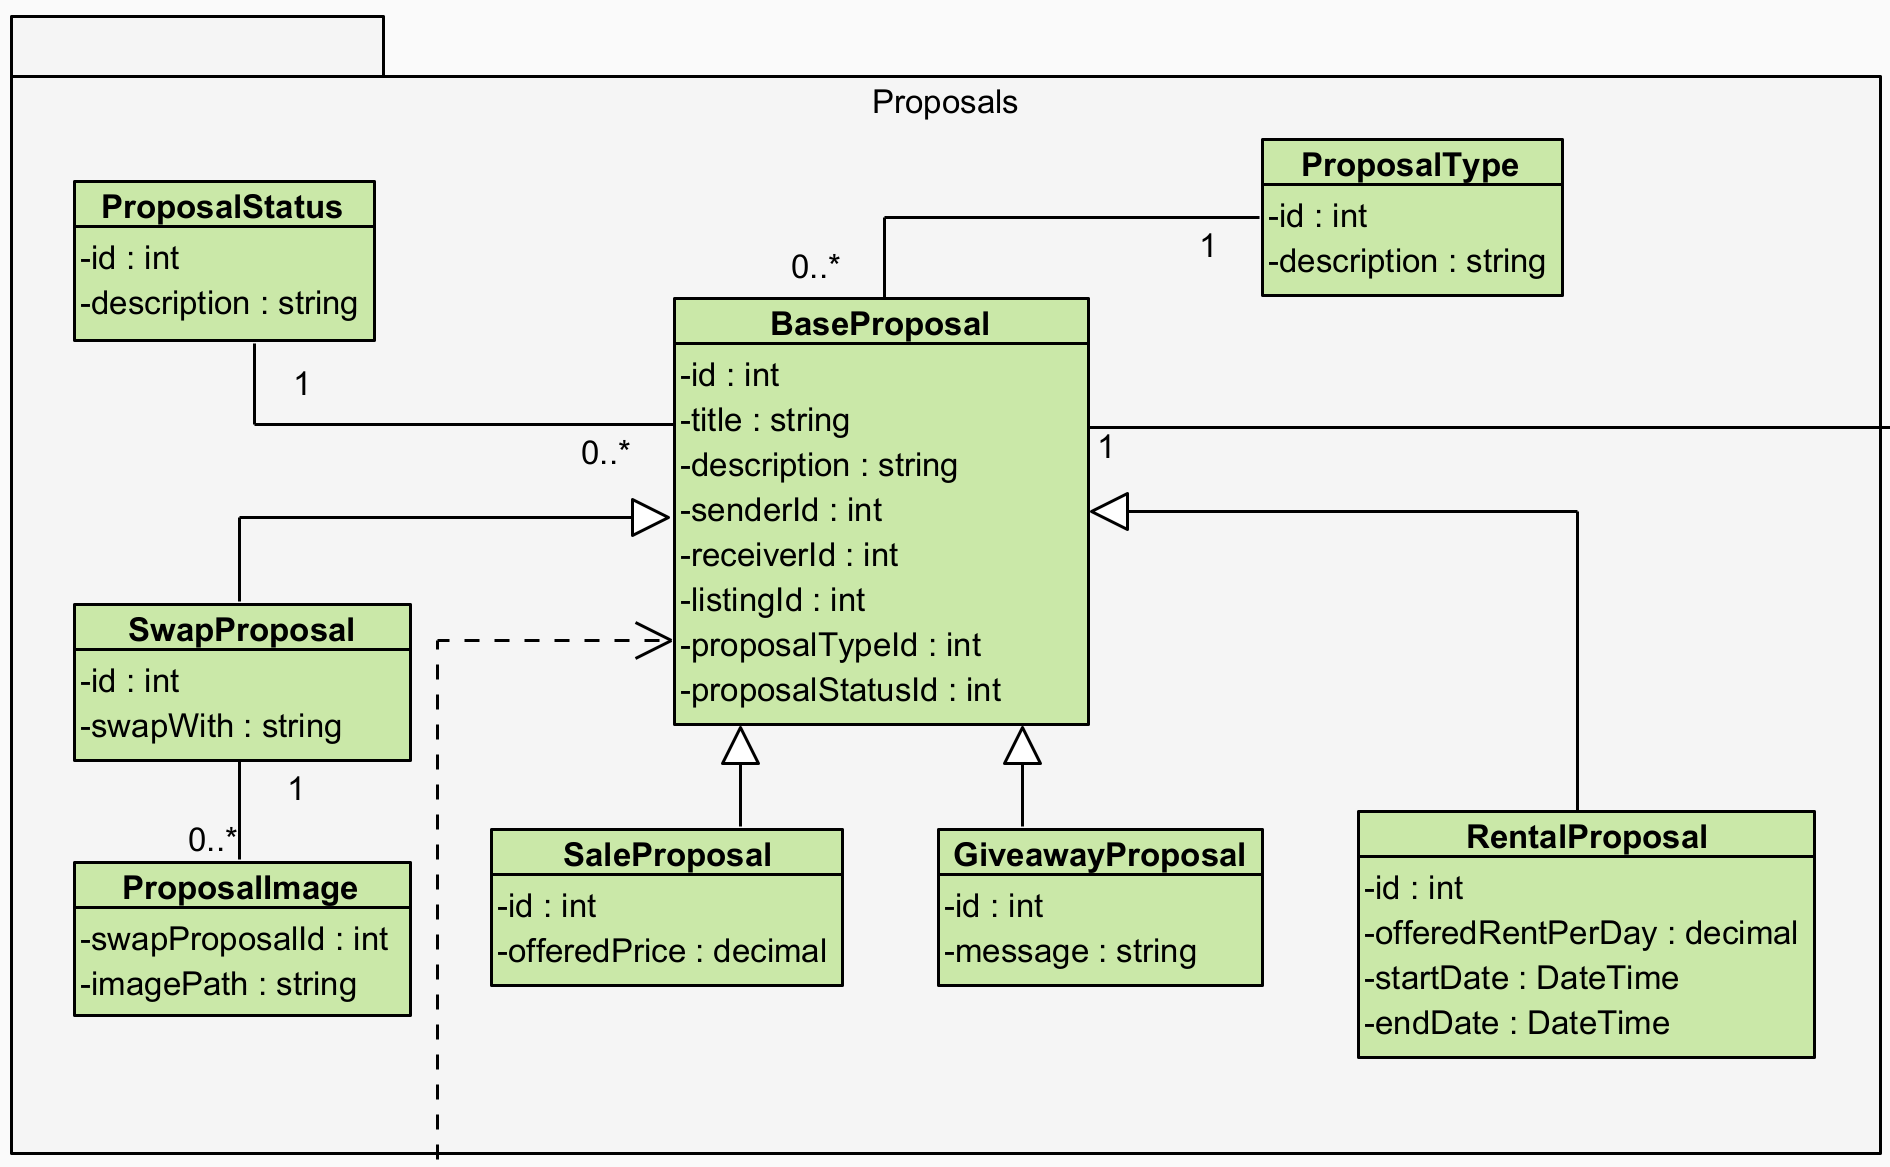
\includegraphics[width=\textwidth]{../images/class-diagram-proposals.png}
	\caption{Diagrama de Classes - Propostas}
	\label{fig:class_diagram_proposals}
\end{figure}

\newpage
\subsection{Transactions}
O pacote \textit{Transactions} é responsável pela gestão das transações entre utilizadores. A classe \textit{Transaction} representa uma transação e guarda a sua data de criação, estado (referenciado pela classe \textit{TransactionStatus}) e o utilizador associado.

A classe \textbf{TransactionStatus} define os estados possíveis de uma transação, com um identificador único e uma descrição textual do estado.

A classe \textbf{UserTransaction} estabelece a relação entre utilizadores e transações, identificando explicitamente o vendedor e o comprador envolvidos numa transação específica. Cada transação pode estar associada a vários registos de \textit{UserTransaction}.

\begin{figure}[ht]
	\centering
	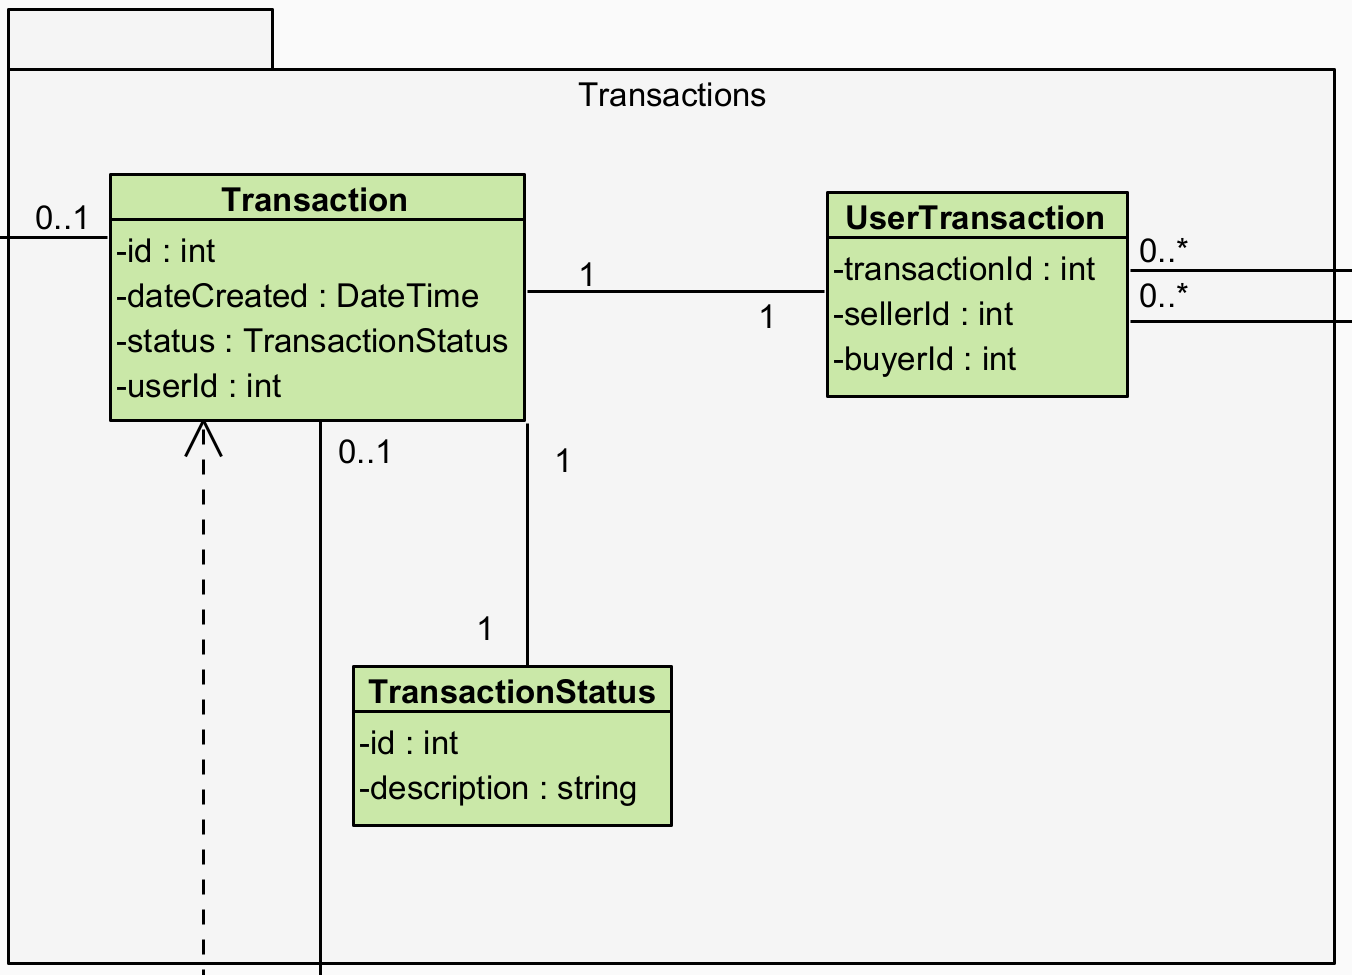
\includegraphics[width=\textwidth]{../images/class-diagram-transactions.png}
	\caption{Diagrama de Classes - Transações}
	\label{fig:class_diagram_transactions}
\end{figure}

\subsection{Product Listings}
O pacote \textit{Product Listings} define os produtos disponíveis na plataforma. A classe \textbf{BaseProductListing} contém atributos comuns a todos os anúncios, como descrição, localização e categoria. Subtipos específicos incluem:
\begin{itemize}
	\item \textbf{SaleListing} - Anúncios para venda, com preço e condição do produto.
	\item \textbf{SwapListing} - Anúncios de troca.
	\item \textbf{GiveawayListing} - Anúncios de oferta gratuita, com requisitos opcionais.
	\item \textbf{RentalListing} - Anúncios de aluguer, incluindo caução e preços.
\end{itemize}
As categorias de produtos são geridas pela classe \textbf{ProductCategory} e as imagens pela classe \textbf{ProductImage}. A disponibilidade para aluguer é gerida pela classe \textbf{RentalAvailability}.

\begin{figure}[ht]
	\centering
	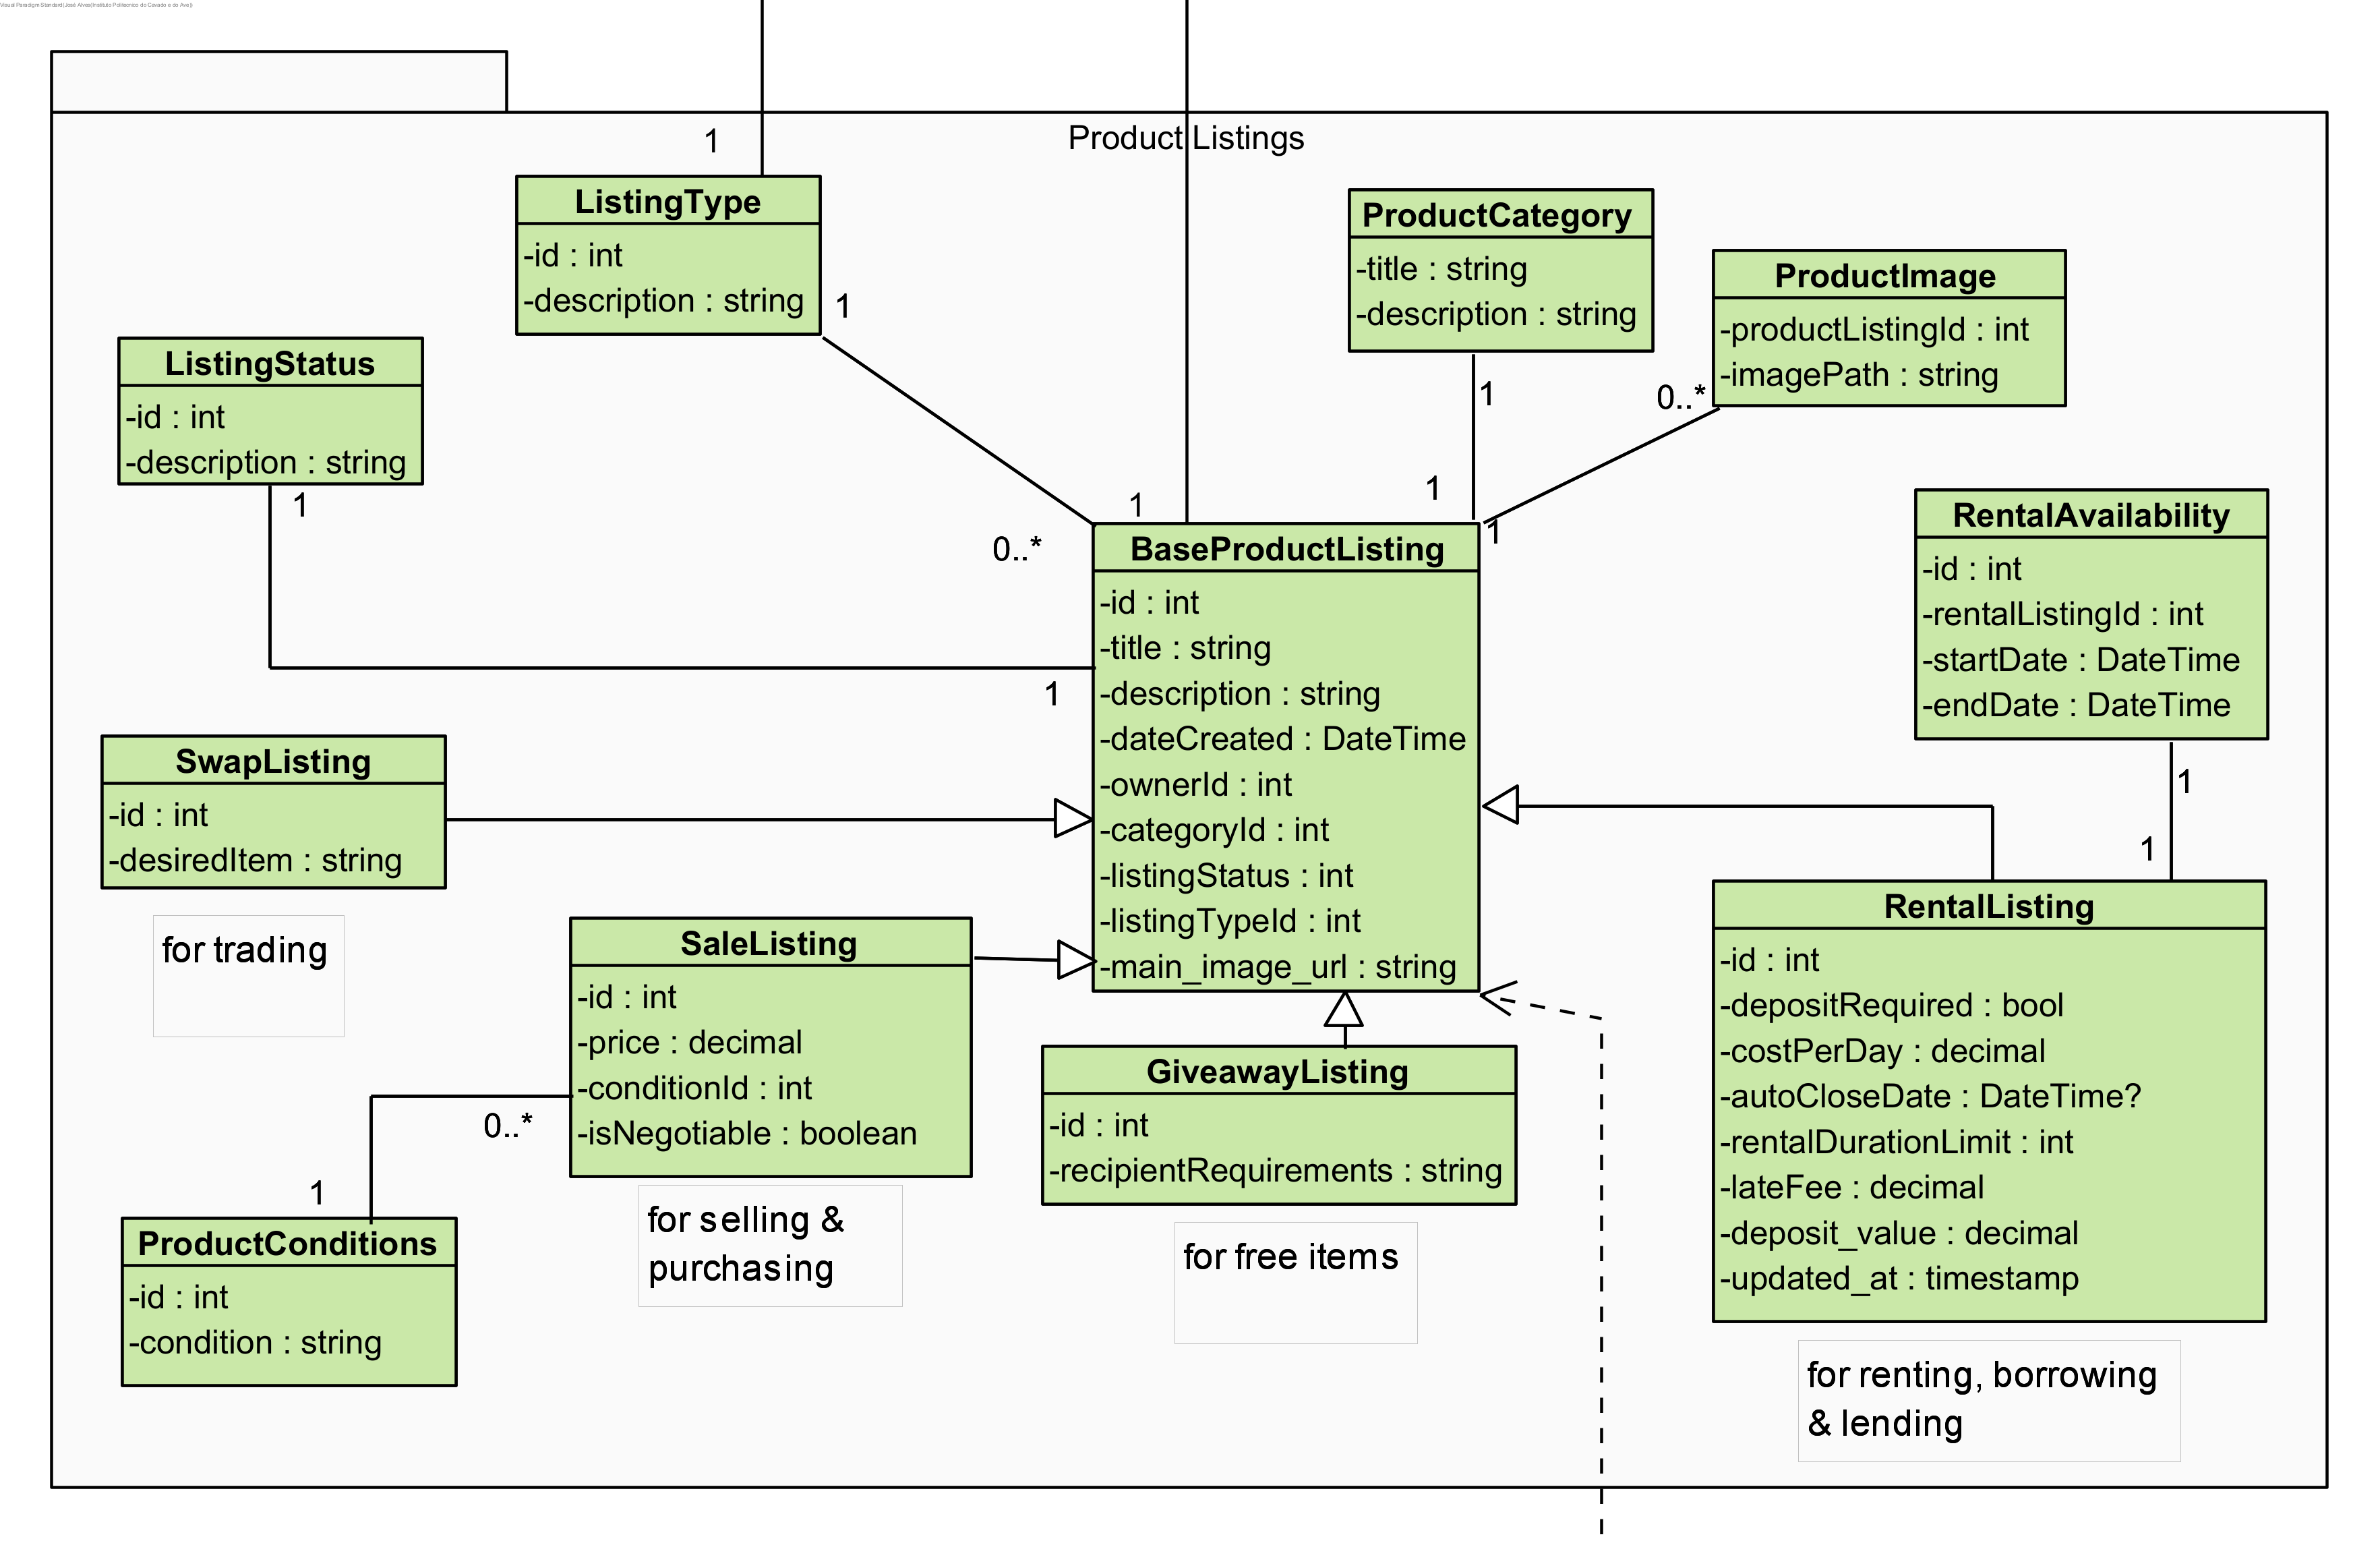
\includegraphics[width=\textwidth]{../images/class-diagram-listings.png}
	\caption{Diagrama de Classes - Anúncios}
	\label{fig:class_diagram_listings}
\end{figure}

\newpage
\subsection{Controladores}
O sistema implementa vários controladores para gerir operações sobre as entidades definidas:
\begin{itemize}
	\item \textbf{ProposalsController} - Gestão de propostas (criação, actualização, aceitação, rejeição).
	\item \textbf{TransactionsController} - Gestão de transacções (criação, actualização, cancelamento).
	\item \textbf{ProductListingsController} - Gestão de anúncios de produtos (criação, actualização, remoção).
	\item \textbf{CategoriesController} - Gestão de categorias de produtos.
	\item \textbf{ImagesController} - Gestão de imagens de produtos.
	\item \textbf{UserController} - Gestão de utilizadores.
	\item \textbf{BlockedUserController} - Gestão de utilizadores bloqueados.
	\item \textbf{FavoritesRepository} - Gestão de favoritos.
	\item \textbf{ContactRepository} - Gestão de contactos.
	\item \textbf{LocationRepository} - Gestão de localizações.
\end{itemize}

Este diagrama e organização asseguram um sistema modular, escalável e bem estruturado para gerir os diferentes aspectos da plataforma.

\begin{figure}[ht]
	\centering
	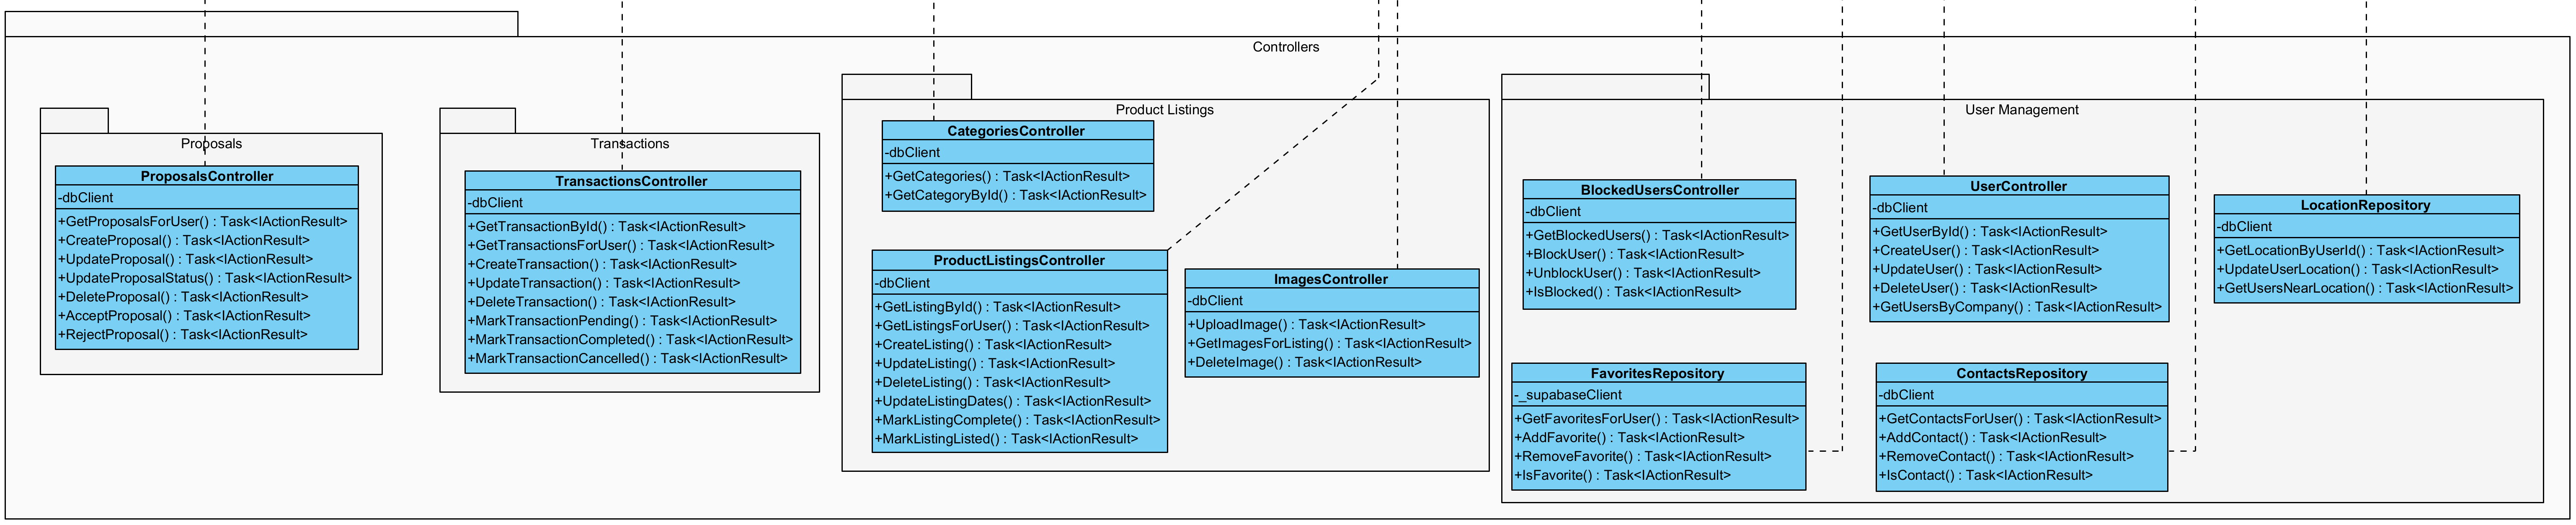
\includegraphics[width=\textwidth]{../images/class-diagram-controllers.png}
	\caption{Diagrama de Classes - Controladores}
	\label{fig:class_diagram_controllers}
\end{figure}

%------------------------------------------------------------------------------------

\newpage
\section{Diagramas de Sequência}

\subsection{Processo de Venda}
O diagrama de sequência apresentado ilustra o fluxo de interações entre os diferentes componentes do sistema no contexto do processo de venda, descrevendo a troca de mensagens e a ordem dos eventos.

Neste cenário, o processo inicia-se quando o utilizador (potencial comprador) acede à aplicação e pesquisa os anúncios nos quais está interessado, desencadeando uma série de chamadas entre os controladores e modelos responsáveis pelo tratamento da informação. A proposta é registada e armazenada na base de dados (PostgreSQL, através do Supabase), podendo posteriormente ser consultada e processada pelo utilizador. Caso a proposta seja aceite, o sistema procede à criação da transação e à atualização do estado do anúncio, concluindo a venda.

\begin{figure}[ht]
	\centering
	\includegraphics[width=\textwidth]{../images/sequence-diagram-sale.png}
	\caption{Diagrama de Sequência do Processo de Venda}
	\label{fig:diagrama_sequencia_venda}
\end{figure}

\subsection{Processo de Troca}
O diagrama de sequência apresentado descreve o fluxo de interações entre os diferentes controladores e modelos envolvidos no processo de troca de produtos. Inicialmente, o utilizador visualiza os anúncios disponíveis, mostrados pelo \textit{ProductListingsController}. Posteriormente, o utilizador pode criar uma proposta de troca, que é submetida e guardada no sistema pelo \textit{ProposalsController}, que por sua vez comunica com o \textit{ProposalsModel}. As propostas recebidas podem ser visualizadas e, caso sejam aceites, o estado da proposta é atualizado. Uma vez aceite a proposta, é iniciada uma transação através do \textit{TransactionsController}, sendo registada e concluída a troca entre os utilizadores. Por fim, o estado do anúncio e da proposta são atualizados para refletir a conclusão da transação, e os contactos dos utilizadores envolvidos são disponibilizados para facilitar a comunicação entre ambos.

\begin{figure}[ht]
	\centering
	\includegraphics[width=\textwidth]{../images/sequence-diagram-swap.png}
	\caption{Diagrama de Sequência do Processo de Troca}
	\label{fig:diagrama_sequencia_troca}
\end{figure}

\subsection{Processo de Aluguer}
O processo de aluguer inicia-se quando o utilizador vai aos anúncios disponíveis e cria uma proposta, que é submetida e armazenada na base de dados.

Após o envio da proposta, o sistema recupera as propostas recebidas e apresenta-as ao proprietário do anúncio. Caso o proprietário aceite a proposta, o estado da mesma é atualizado e uma transação é criada através do \textit{TransactionsController}. Esta é então processada e dada como concluída.

Além disso, os dados do anúncio são atualizados para refletir a alteração no estado de disponibilidade do produto. Os utilizadores podem posteriormente visualizar o estado das suas propostas e, caso necessário, aceder aos contactos da outra parte envolvida no aluguer, disponibilizados pelo \textit{ContactsController}.

Este processo assegura que o aluguer ocorre de forma controlada e registada, garantindo que tanto o proprietário quanto o cliente tenham acesso a informações relevantes durante toda a transação.

\begin{figure}[ht]
	\centering
	\includegraphics[width=\textwidth]{../images/sequence-diagram-rental.png}
	\caption{Diagrama de Sequência do Processo de Aluguer}
	\label{fig:diagrama_sequencia_aluguer}
\end{figure}

%------------------------------------------------
\newpage
\section{Diagrama de Atividades}

Os diagramas de atividade representam o fluxo de operações dentro de um sistema, destacando as ações realizadas e a interação entre os participantes. Eles são utilizados para modelar processos, ilustrando a sequência de atividades, decisões e possíveis caminhos alternativos. No contexto deste sistema, os diagramas de atividade descrevem os processos de vendas, aluguer e trocas, facilitando a compreensão do funcionamento e das etapas envolvidas.

\subsection{Processo de Troca}
O processo de troca inicia-se quando um cliente está interessado num item e propõe uma troca ao seu dono. O fluxo segue da seguinte forma:

\begin{itemize}
	\item O cliente, interessado num item, envia uma proposta de troca ao dono do item.
	\item O dono recebe a proposta e pode:
	\begin{itemize}
		\item Aceitar a proposta, concluindo a troca.
		\item Rejeitar a proposta, encerrando o processo.
		\item Criar uma contraproposta se tomou a decisão de negociar.
	\end{itemize}
	\item Se o dono criar uma contraproposta:
	\begin{itemize}
		\item O cliente pode aceitar a contraproposta, realizando a troca.
		\item O cliente pode rejeitar a contraproposta, encerrando o processo.
		\item O cliente pode optar por continuar a negociar, enviando uma nova proposta.
	\end{itemize}
	\item O processo continua até que uma proposta seja aceite por ambas as partes ou até que uma das partes decida encerrar a negociação.
\end{itemize}

\begin{figure}[ht]
	\centering
	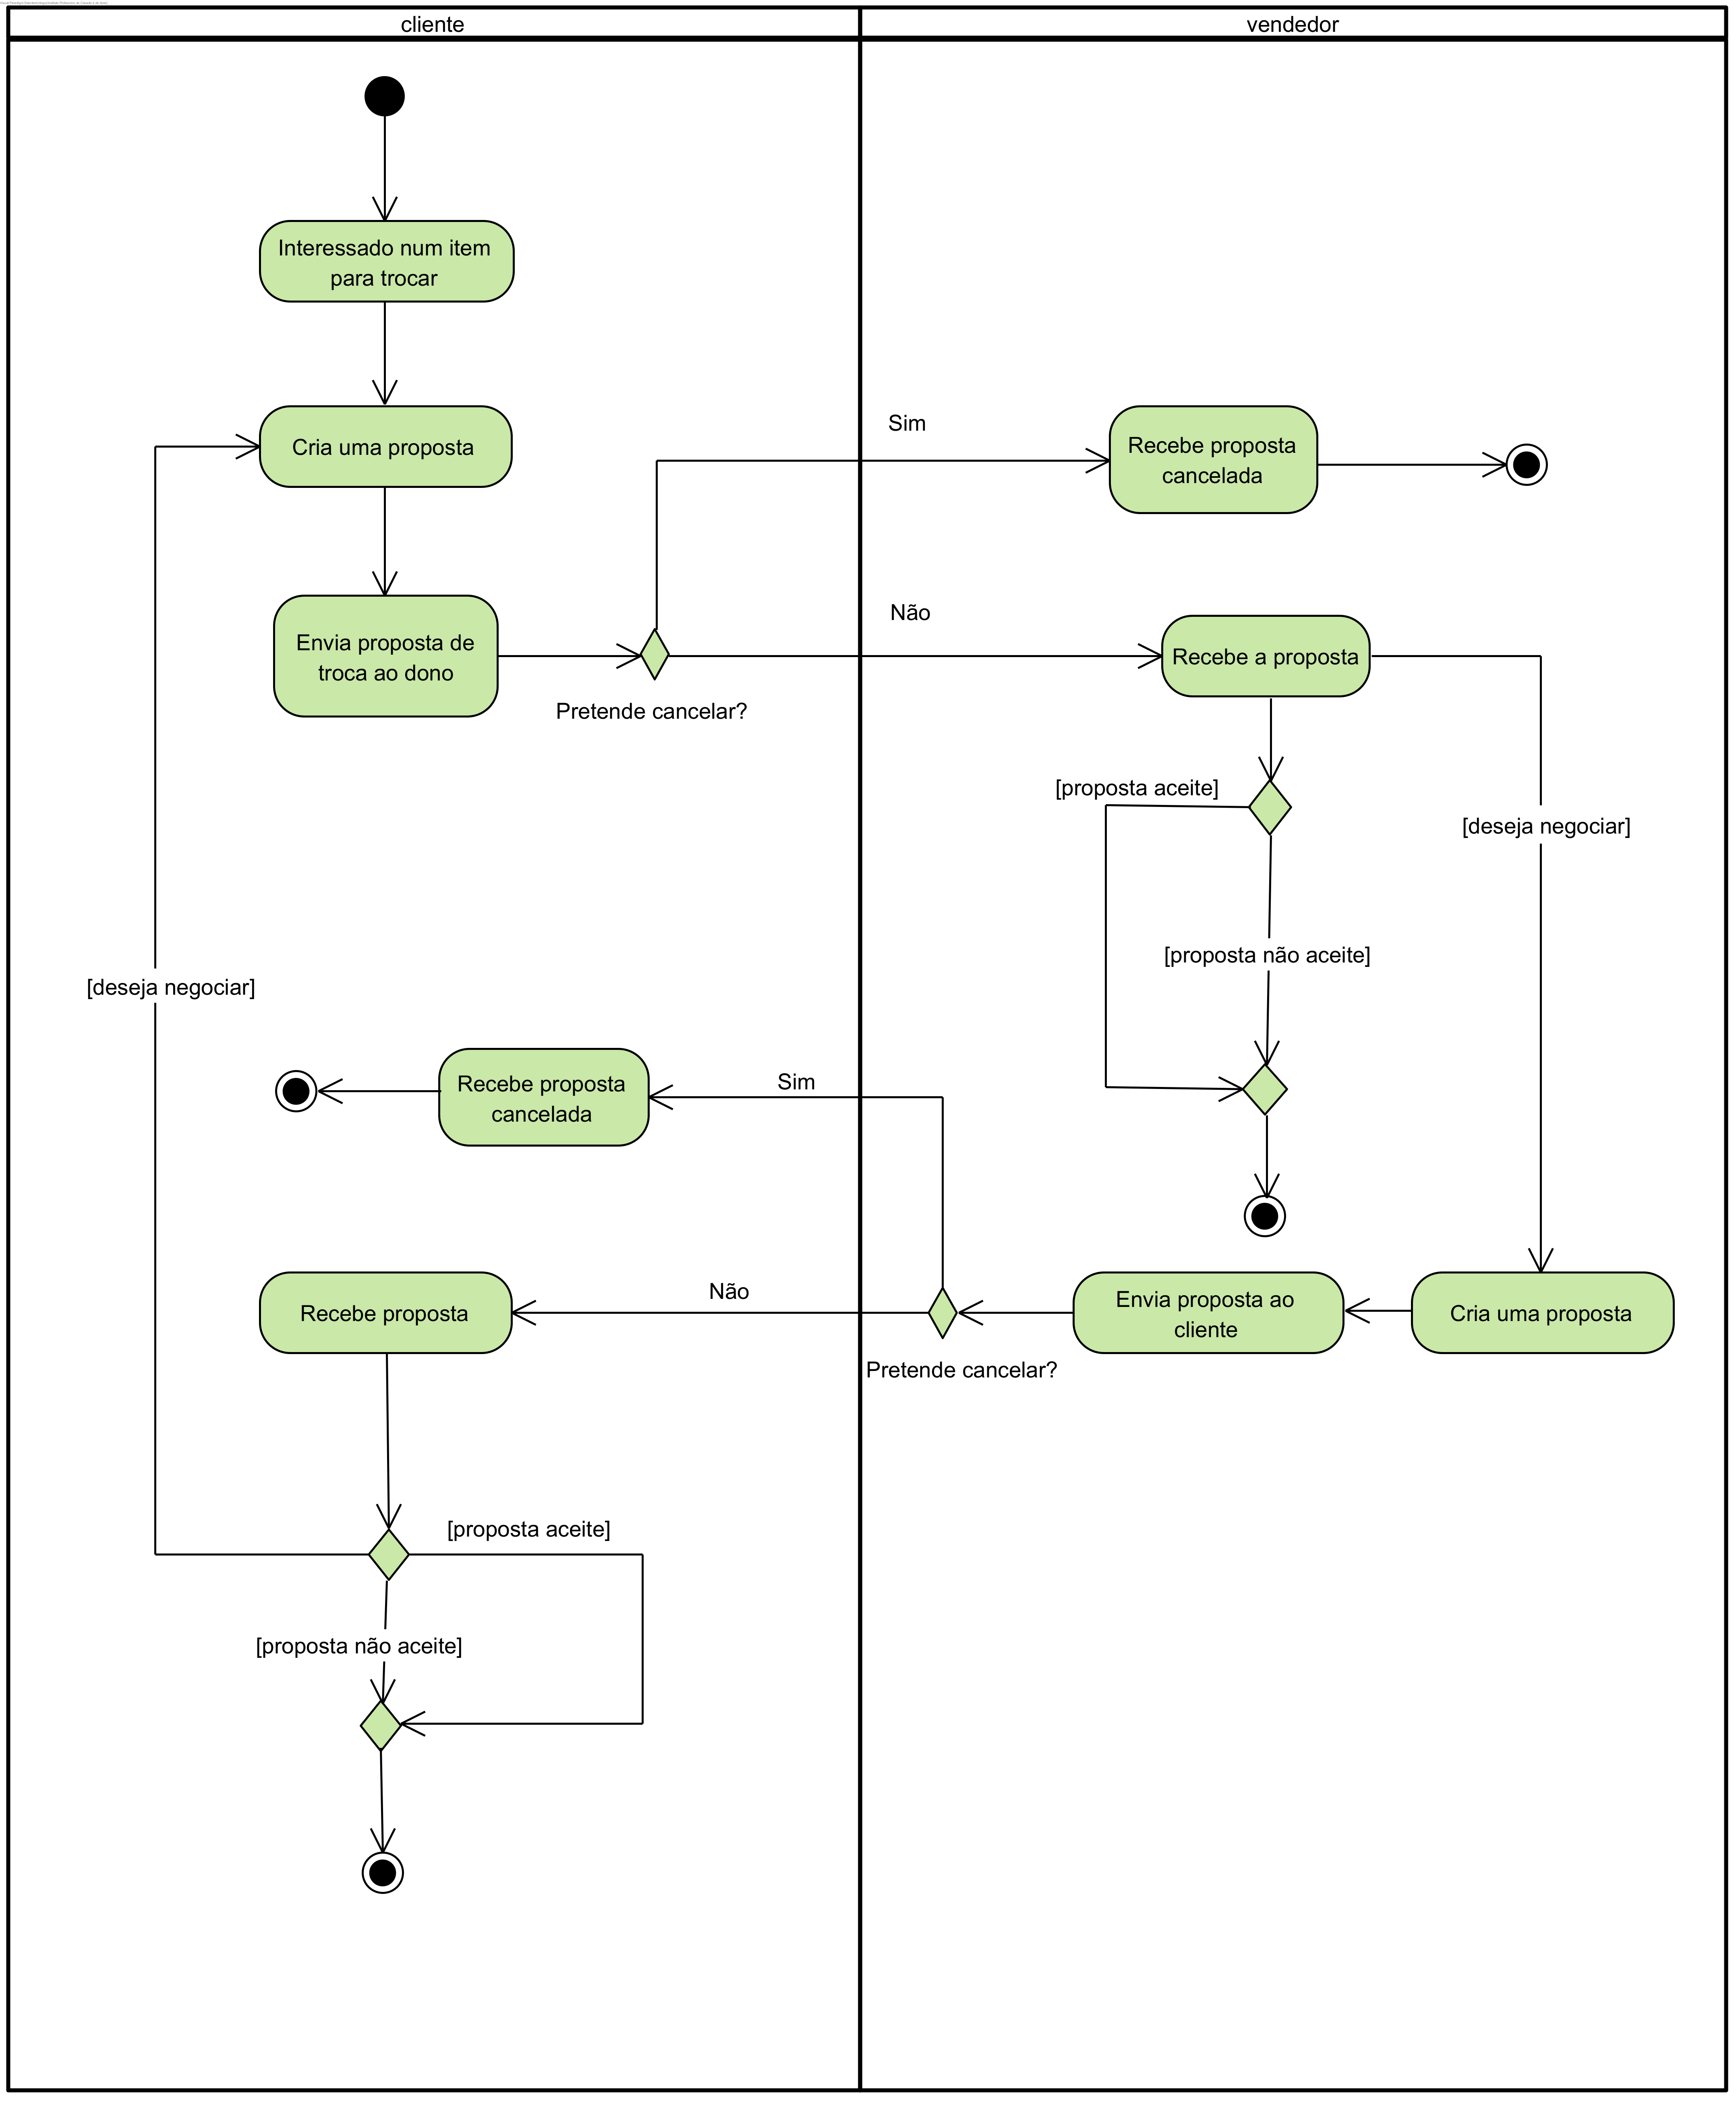
\includegraphics[width=0.8\textwidth]{../images/activity-diagram-swaps.png}
	\caption{Diagrama de atividades do Processo de Troca}
	\label{fig:diagrama_atividades_troca}
\end{figure}

%------------------------------------------------
\newpage
\clearpage

\subsection{Processo de Venda}
O processo de venda inicia-se quando um cliente está interessado em comprar um item. O fluxo segue da seguinte forma:

\begin{itemize}
	\item O cliente, interessado em comprar um item, verifica se o item é negociável.
	\begin{itemize}
		\item Se o item não for negociável, o cliente pode aceitar as condições de venda ou desistir da compra.
		\item Se o item for negociável, o cliente pode enviar uma proposta de compra ao vendedor.
	\end{itemize}
	\item O vendedor recebe a proposta e pode:
	\begin{itemize}
		\item Aceitar a proposta, concluindo a venda.
		\item Rejeitar a proposta, encerrando o processo.
		\item Criar uma contraproposta para continuar a negociação.
	\end{itemize}
	\item Se o vendedor criar uma contraproposta:
	\begin{itemize}
		\item O cliente pode aceitar a contraproposta, concluindo a venda.
		\item O cliente pode rejeitar a contraproposta, encerrando o processo.
		\item O cliente pode optar por continuar a negociar, enviando uma nova proposta.
	\end{itemize}
	\item O processo de negociação continua até que:
	\begin{itemize}
		\item Ambas as partes cheguem a um acordo, concluindo a venda.
		\item Uma das partes decida encerrar a negociação.
	\end{itemize}
	\item Caso um acordo seja alcançado, a venda é concluída e o item é entregue ao cliente.
\end{itemize}

\begin{figure}[ht]
	\centering
	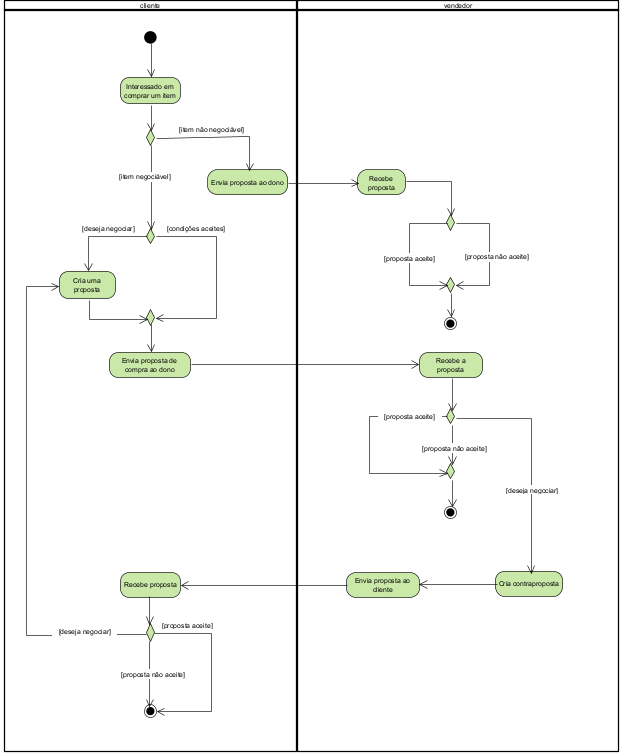
\includegraphics[width=0.8\textwidth]{../images/activity-diagram-sales.png}
	\caption{Diagrama de atividades do Processo de Vendas}
	\label{fig:diagrama_atividades_vendas}
\end{figure}
%------------------------------------------------
\newpage
\clearpage

\subsection{Processo de Aluguer}
O processo de aluguer inicia-se quando um cliente está interessado em alugar um item. O fluxo segue da seguinte forma:

\begin{itemize}
	\item O cliente, interessado em alugar um item, verifica as condições de aluguer.
	\begin{itemize}
		\item Se as condições forem aceites, o cliente pode prosseguir com o aluguer.
		\item Se o cliente desejar negociar, pode criar uma contraproposta e enviá-la ao dono do item.
	\end{itemize}
	\item O dono do item recebe a proposta e pode:
	\begin{itemize}
		\item Aceitar a proposta, concluindo o acordo de aluguer.
		\item Rejeitar a proposta, encerrando o processo.
		\item Criar uma contraproposta para continuar a negociação.
	\end{itemize}
	\item Se o dono criar uma contraproposta:
	\begin{itemize}
		\item O cliente pode aceitar a contraproposta, concluindo o aluguer.
		\item O cliente pode rejeitar a contraproposta, encerrando o processo.
		\item O cliente pode optar por continuar a negociar, enviando uma nova proposta.
	\end{itemize}
	\item O processo de negociação continua até que:
	\begin{itemize}
		\item Ambas as partes cheguem a um acordo, concluindo o aluguer.
		\item Uma das partes decida encerrar a negociação.
	\end{itemize}
	\item Caso um acordo seja alcançado, o aluguer é registado no sistema.
\end{itemize}

\begin{figure}[ht]
	\centering
	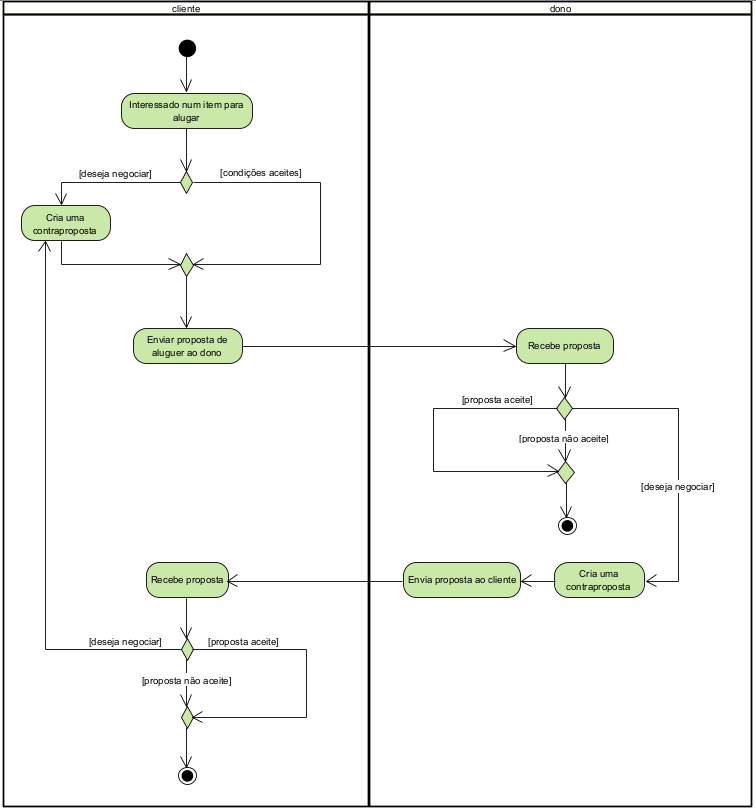
\includegraphics[width=0.8\textwidth]{../images/activity-diagram-rentals.png}
	\caption{Diagrama de atividades do Processo de Aluguer}
	\label{fig:diagrama_atividades_aluguer}
\end{figure}

%------------------------------------------------

\newpage
\clearpage
\section{Design UI}
A interface do utilizador (UI) da plataforma foi concebida para proporcionar uma experiência visual agradável e coerente, garantindo uma navegação intuitiva e acessível. Os mockups desenvolvidos ilustram o design das páginas, incluindo a organização dos elementos, a paleta de cores, a tipografia e os componentes interativos.

Para consulta detalhada dos mockups e da estrutura visual da plataforma, estes estão disponíveis numa pasta anexada a este relatório.

\begin{figure}[ht]
	\centering
	\includegraphics[width=\textwidth]{../images/mockup-laptop.png}
	\caption{Mockup da aplicação}
	\label{fig:mockup}
\end{figure}

%------------------------------------------------

\newpage
\section{\textit{Milestones}}
O desenvolvimento da plataforma seguirá uma abordagem faseada, garantindo um planeamento estruturado e entregas progressivas ao longo do processo. Para assegurar um acompanhamento claro do progresso, foram definidos marcos essenciais que representam as principais fases do projeto.

\subsection{Planeamento e Entregas}

As etapas-chave do desenvolvimento e as respetivas datas de entrega são as seguintes:

\begin{itemize}
	\item \textbf{Entrega da Especificação} \textit{(9 de março de 2025)} – Nesta fase, será elaborado e entregue o documento de especificação do projeto, contendo a definição dos requisitos funcionais e não funcionais, bem como a arquitetura do sistema e os principais diagramas UML.
	
	\item \textbf{Fase \textit{Alpha}} \textit{(6 de abril de 2025)} – Esta versão irá corresponder ao primeiro protótipo funcional da aplicação. O foco está em seguir a arquitetura e integrar os principais componentes.
	
	\item \textbf{Versão \textit{Beta}} \textit{(20 de abril de 2025)} – Com base no feedback da fase Alpha, esta versão tem como objetivo incorporar melhorias gerais da aplicação. Além disso, serão realizados testes mais aprofundados, abrangendo diferentes cenários de utilização para garantir estabilidade e usabilidade.
	
	\item \textbf{Versão RTW (\textit{Ready to Web})} \textit{(11 de maio de 2025)} – Esta versão representará a aplicação finalizada, pronta para disponibilização ao público. Nesta fase, serão concluídas as últimas correções, ajustes de funcionalidades e serão realizadas as validações finais para assegurar a conformidade com os objetivos do projeto.
\end{itemize}

A definição destes marcos permitirá uma gestão eficiente do desenvolvimento, garantindo que cada etapa seja devidamente planeada, implementada e validada antes do avanço para a fase seguinte.

%------------------------------------------------
\newpage
\section{Conclusão}

A plataforma proposta tem como objetivo criar um ambiente seguro e eficiente para a troca, venda e empréstimo de produtos dentro de uma comunidade. Ao permitir a marcação de encontros para a realização das transações, o projeto fomenta a interação entre os membros e incentiva práticas de consumo consciente. 
Com a definição clara dos requisitos e o suporte de diagramas UML e mockups, este relatório serve como um guia para o desenvolvimento da solução, garantindo que todos os aspectos essenciais sejam considerados.

\newpage
%----------------------------------------------------------------------------------------
%	BIBLIOGRAPHY
%----------------------------------------------------------------------------------------
\nocite{*}

\printbibliography
%----------------------------------------------------------------------------------------

\end{document}